% Source-derived chapter 08: Invariance properties
% Original source: pixtons-formula-abel-jacobi-picard-stack
\chapter{Invariance properties}
\label{pixtons-formula-abel-jacobi-picard-stack-chapter-08}
\source{pixtons-formula-abel-jacobi-picard-stack}

\begin{remark}[Source section]
\label{pixtons-formula-abel-jacobi-picard-stack-chapter-08-source}
\source{pixtons-formula-abel-jacobi-picard-stack}
\source{pixtons-formula-abel-jacobi-picard-stack}
This chapter reproduces the corresponding section of the retrieved
LaTeX source, including its definitions, statements, examples, and
proofs. It has not yet been translated into Lean.
\notready
\end{remark}

% The source section title was: Invariance properties
\label{Sect:proofInvariance}
\source{pixtons-formula-abel-jacobi-picard-stack}
\subsection{Overview}
We prove here the invariance properties of the universal twisted double ramification cycle as presented in Section \ref{Sect:introinvariance}. 

We start with an object of $\phi_\ca L\colon \mathcal S \to \Picabs_{g,n,d}$ 
given by
a flat family of prestable $n$-pointed genus $g$ curves together with a line bundle of relative degree $d$,
    \begin{equation}
    \label{eqn:invSobj}    
\source{pixtons-formula-abel-jacobi-picard-stack}
    \pi:\mathcal{C} \rightarrow \mathcal{S}\, , \ \ \ \ p_1,\ldots,p_n: \mathcal{S} \rightarrow \mathcal{C}\, , \ \ \ \
        \mathcal{L} \rightarrow \mathcal{C}\, .
        \end{equation}
    Let $\mathsf{DR}^{\mathsf{op}}_{g,A,\mathcal{L}}= \phi_\ca L^*\DRop_{g,A}\in \mathsf{CH}^g_{\mathsf{op}}(\mathcal{S})$
    be the twisted double ramification cycle associated to the above
    family \eqref{eqn:invSobj} and
     the vector
    $$A=(a_1,\ldots, a_n)\, , \ \ \ \ d =\sum_{i=1}^n a_i\, .$$

%In Section  \ref{Sect:introinvariance} several invariance properties of   $\mathsf{DR}^{\mathsf{op}}_{g,A,\mathcal{L}}$ were discussed. 

Theorem \ref{Thm:main} asserts that  $\DRop_{g,A}$ is equal to
the tautological class
$$\P^g_{g,A,d} \in \CHop^g(\Picabs_{g,n,d})\, .$$ If we
assume Theorem \ref{Thm:main}, we have a choice of proving the invariance properties either for $\DRop_{g,A}$ or for the formula in tautological classes. In fact, since both
sides of Invariances \invnrn, \invnrA{} and
\invnrIV{} are used {\em in the proof} of Theorem \ref{Thm:main},
we will have to prove these two sides separately in each of these cases. 
In fact, we will do this for all the invariances, as each side yields interesting perspectives. Also, we will show the invariances of Pixton's formula hold
not just for 
the codimension $g$ part $\P^g_{g,A,d}$, but for the full mixed degree class
\[\P^\bullet_{g,A,d} \in \prod_{c=0}^\infty \CHop^c(\Picabs_{g,n,d})\, .\]

%One thing to note is that $\mathsf{DR}^{\mathsf{op}}_{g,A,\mathcal{L}}$ is the pullback of the universal twisted double ramification cycle on $\Picabs_{g,n,d}$, for which we showed a formula in the tautological ring of $\Picabs_{g,n,d}$. Thus it is possible to either show the invariance of $\mathsf{DR}^{\mathsf{op}}_{g,A,\mathcal{L}}$ directly from the definition, or alternatively show that this tautological formula has the desired invariance property. We will give both perspectives below.

\subsection{Proof of Invariance \invnrI{}: {\rm Dualizing}}
We want to show the invariance
        $$\mathsf{DR}^{\mathsf{op}}_{g,-A, \mathcal{L}^*}
        =\epsilon^* \mathsf{DR}^{\mathsf{op}}_{g,A, \mathcal{L}}
        \, , $$
where $\epsilon: \Picabs_{g,n,-d} \rightarrow \Picabs_{g,n,d}$
is the natural map obtained via dualizing the line bundle.  It is enough to show the invariance
\begin{equation}\label{vv99q}
\source{pixtons-formula-abel-jacobi-picard-stack}
\mathsf{DR}^{\mathsf{op}}_{g,-A} = \epsilon^* \mathsf{DR}^{\mathsf{op}}_{g,A}
\end{equation}
of the universal twisted double ramification cycles.
The invariance \eqref{vv99q} can be deduced by applying \cref{lem:pushpullcommutes} to the following commutative diagram of morphisms, where the horizontal morphisms are the corresponding Abel-Jacobi maps and the vertical morphisms are isomorphisms
\[\begin{tikzcd}
\cat{Div}_{g,A} \arrow[r] \arrow[d, "\widehat \epsilon"] &\Picabs_{g,n,d} \arrow[d,"\epsilon"]\\
\cat{Div}_{g,-A} \arrow[r]  &\, \Picabs_{g,n,-d}\, .
\end{tikzcd}
\]
Here, in the language of Section \ref{sec:log_def}, the morphism $\widehat \epsilon$ is induced by the natural map $\pi_*\bar M_C^{gp}/\bar M_S^{gp} \to \pi_*\bar M_C^{gp}/\bar M_S^{gp}$ given by inversion in $\bar M_C^{gp}$. \qed

We now prove the invariance 
\begin{equation}\label{ww99}
\source{pixtons-formula-abel-jacobi-picard-stack}
\P_{g,-A,-d}^\bullet = \epsilon^*\P_{g,A,d}^\bullet
\end{equation}
using the formulas for these cycles from \cref{Lem:Pixformulafactorization}. The equality is then implied by the following observations:
\begin{itemize}
\item We write  $\ca L_A = \ca L(- \sum_{i=1}^n a_i p_i)$ for the twisted universal line bundle on the universal curve $\pi: \frak C \to \Picabs_{g,n,d}$, and we use \cref{Lem:vertterm} to obtain
\begin{align*}
    \epsilon^* \left(-\eta + \sum_{i=1}^n 2 a_i \xi_i+ a_i^2 \psi_i \right) &= - \epsilon^* \pi_* c_1(\mathcal{L}_A)^2 = - \pi_* c_1((\mathcal{L}_A)^*)^2\\ &= - \pi_* (-c_1(\mathcal{L}_A))^2= - \pi_* c_1(\mathcal{L}_A)^2\\
    &=-\eta + \sum_{i=1}^n 2 a_i \xi_i+ a_i^2 \psi_i\, .
\end{align*}
\item Given a prestable graph $\Gamma_\delta$ describing a stratum in $\Picabs_{g,n,-d}$, the map $\epsilon$ sends this stratum isomorphically to the stratum of $\Gamma_{-\delta}$ (with an associated commutative diagram of gluing morphisms over $\frak M_{g,n}$). Combined with the equality $c_A(\Gamma_\delta) = c_{-A}(\Gamma_{-\delta})$ for $\Gamma_\delta \in \G_{g,n,d}^\textup{se}$ , we see  that the first line of formula \eqref{eqn:Pixformulafactorization} for $\P_{g,A,d}^\bullet$ has the desired invariance.
\item For the sum over graphs and weightings, we clearly have $h^1(\Gamma_\delta) = h^1(\Gamma_{-\delta})$ and $\Aut(\Gamma_\delta)=\Aut(\Gamma_{-\delta})$. Moreover, we have a natural bijection of the admissible weightings modulo $r$
\[\mathsf{W}_{\Gamma_\delta,r} \to \mathsf{W}_{\Gamma_{-\delta},r}\, , \ \ \ w \mapsto (h \mapsto r-w(h) \ \text{mod}\ r).\]
The  map of weightings leaves the edge terms of the formula \eqref{eqn:Pixformulafactorization} invariant  since they only depend on products $w(h)w(h')$ for and edge $(h,h')$ --  which are of the form $a(r-a)$ and thus sent to $(r-a)a$.
\end{itemize}
Therefore, the formula of Proposition \ref{Lem:Pixformulafactorization} applied to 
the two sides of \eqref{ww99} yields the same result. \qed


% We now prove the invariance $\P_{g,-A,-d}^g = \epsilon^*\P_{g,A,d}^g$. Given a prestable graph $\Gamma_\delta$ describing a stratum in $\Picabs_{g,n,-d}$, the map $\epsilon$ sends this stratum isomorphically to the stratum of $\Gamma_{-\delta}$ (with an associated commutative diagram of gluing morphisms over $\frak M_{g,n}$). We also have a natural bijection of the admissible weightings $\mathsf{W}_{\Gamma_\delta,r}$ modulo $r$
% \[\mathsf{W}_{\Gamma_\delta,r} \to \mathsf{W}_{\Gamma_{-\delta},r}, w \mapsto (h \mapsto r-w(h) \mod r).\]
% This leaves the edge-term of the formula of $\P_{g,A,d}^g$ invariant, since it only depends on products $w(h)w(h')$ for $h,h'$ forming an edge, which are anyway of the form $a(r-a)$.
% On the other hand, for the vertex-term we have
% \[\epsilon^* \exp\left(\frac{1}{2} \eta \right) =  \exp\left(\frac{1}{2} \pi_* c_1( \mathcal{L}^*)^2 \right) = \exp\left(\frac{1}{2} \pi_* \left( - c_1(\mathcal{L})\right)^2 \right) = \exp\left(\frac{1}{2} \pi_* c_1(\mathcal{L})^2 \right),\]
% Likewise, for the leg-term we have
% \[\epsilon^* \exp\left(\frac12 a_i^2 \psi_i + a_i \xi_i \right) =  \exp\left(\frac12 a_i^2 \psi_i + a_i p_i^*(c_1(\mathcal{L}^*)) \right)=  \exp\left(\frac12 (-a_i)^2 \psi_i + (-a_i) \xi_i \right),\]
% thus this part of the formula is also invariant.

\subsection{Proof of Invariance \invnrn{}: {\rm Unweighted markings}}
Assume we have an additional section $p_{n+1}: \mathcal{S} \rightarrow \mathcal{C}$ of $\pi$ which yields an object of $\Picabs_{g,n+1,d}$,
    \begin{equation}
    \label{ff44996}    
\source{pixtons-formula-abel-jacobi-picard-stack}
    \pi:\mathcal{C} \rightarrow \mathcal{S}\, , \ \ \ \ p_1,\ldots,p_n,p_{n+1}: \mathcal{S} \rightarrow \mathcal{C}\, , \ \ \ \
        \mathcal{L} \rightarrow \mathcal{C}\, .
        \end{equation}
 Then, for the vector $A_0 \in \mathbb{Z}^{n+1}$ obtained by appending $0$ (as the last coefficient) to $A$, we want to show the invariance
 \begin{equation} \label{eqn:n_invar_repeat}
\source{pixtons-formula-abel-jacobi-picard-stack}
     \mathsf{DR}^{\mathsf{op}}_{g,A_0, \mathcal{L}}
        =\mathsf{DR}^{\mathsf{op}}_{g,A, \mathcal{L}}
        \, .
 \end{equation}



For the map
$\frak M_{g,n+1} \to \frak M_{g,n}$
induced by forgetting the last marking, we have a diagram of cartesian squares
\begin{equation}
 \begin{tikzcd}
  \cat{Div}_{g,A_0} \arrow[r]\arrow[d]  & \cat{Div}_{g,A} \arrow[d]\\
  \Picabs_{g,n+1,d} \arrow[r,"F"] \arrow[d] & \Picabs_{g,n,d} \arrow[d]\\
  \frak M_{g, n+1} \arrow[r] & \frak M_{g,n}\, , 
\end{tikzcd}
\end{equation}
where the morphism $F$ is syntomic. In particular, for $\bd 0 \in \mathbb{Z}^n$ the zero vector, the stack $\cat{Div}_{g, \bd 0}$ can be obtained by pulling back
%\footnote{\{Here $[]$ denotes a vector of length 0. I have no idea what notation we want for this!} Y: We used $\DRop_{g,\emptyset}$ in \cref{sec:intro_deg_0}, so $\emptyset$ might be an option. \jocomment{What about writing just $\cat{Div}_{g}$?
%R: I think we shouldnt have more notation! We already have the emptyset which makes %complete %sense here.}} 
$\cat{Div}_{g,\emptyset}$ from $\Picabs_{g,0,0}$. 
Then, as a consequence of the above cartesian square and the
definition of the double ramification cycle, \cref{lem:pushpullcommutes} yields
\begin{equation} \label{eqn:DR_forget_pullback}
\source{pixtons-formula-abel-jacobi-picard-stack}
    F^* \mathsf{DR}^{\mathsf{op}}_{g,A} = \mathsf{DR}^{\mathsf{op}}_{g,A_0}\ .
\end{equation}
Since the morphisms $\ca S \to \Picabs_{g,n,d}$ and $\ca S \to \Picabs_{g,n+1,d}$ used to define $\mathsf{DR}^{\mathsf{op}}_{g,A, \mathcal{L}}$ and $\mathsf{DR}^{\mathsf{op}}_{g,A_0, \mathcal{L}}$ fit in a diagram
\[
\begin{tikzcd}
\ca S \arrow[d] \arrow[dr]& \\
\Picabs_{g,n+1,d} \arrow[r,"F"] & \Picabs_{g,n,d}
\end{tikzcd}
\]
the equation \eqref{eqn:DR_forget_pullback} immediately proves the invariance \eqref{eqn:n_invar_repeat}. \qed

% \begin{lemma} \label{Lem:DR_forget_pullback}
% The operational class $\in \mathsf{CH}_{\mathsf{op}}^g(\Picabs_{g,n+1,d})$ is the pullback
% of $\in \mathsf{CH}_{\mathsf{op}}^g(\Picabs_{g,n,d})$
% under the forgetful map $F$.
% \end{lemma}

We now prove the corresponding invariance
\begin{equation} \label{eqn:P_forget_pullback}
\source{pixtons-formula-abel-jacobi-picard-stack}
    F^* \P_{g,A,d}^\bullet = \P_{g,A_0,d}^\bullet\ 
\end{equation}
% \begin{lemma} \label{wwwrrr}
% The class $\P_{g,A_0,d}^\bullet$ is the pullback
% of $\P_{g,A,d}^\bullet$
% under the forgetful map $F$.
% \end{lemma}
% \begin{proof}
of Pixton's formula. First, since the map $F$ does not change the curve or the line bundle, we have a Cartesian diagram
\[
\begin{tikzcd}
\frak C_{g,n+1,d} \arrow[r,"\widehat{F}"] \arrow[d,"\pi'"]& \frak C_{g,n,d} \arrow[d,"\pi"]\\
\Picabs_{g,n+1,d} \arrow[r,"{F}"]& \Picabs_{g,n,d}\, .
\end{tikzcd}
\]
The universal line bundles $\ca L_{g,n,d}$ and $\ca L_{g,n+1,d}$ on $\frak C_{g,n,d}$ and $\frak C_{g,n+1,d}$ satisfy  $$\widehat{F}^* \ca L_{g,n,d} = \ca L_{g,n+1,d}\, .$$ Similarly, for the canonical line bundles of $\pi, \pi'$ we have $\widehat{F}^* \omega_\pi = \omega_{\pi'}$. Combining these facts, we see that $F$ pulls back the operational
classes $\eta, \xi_i, \psi_i$ on $\Picabs_{g,n,d}$ 
%(for $i=1, \ldots, n$) 
to the corresponding classes on $\Picabs_{g,n+1,d}$.

Next, given a graph $\Gamma_\delta \in \G_{g,n,d}$, we have a fibre diagram
\begin{equation} \label{eqn:forgetgluefibre}
\source{pixtons-formula-abel-jacobi-picard-stack}
\begin{tikzcd}
 \coprod_{v \in \V(\Gamma)} \Picabs_{\Gamma_{v,\delta}} \arrow[r,"\coprod_v j_{\Gamma_{v,\delta}}"] \arrow[d] & \Picabs_{g,n+1,d} \arrow[d,"\pi"]\\
 \Picabs_{\Gamma_{\delta}} \arrow[r,"j_{\Gamma_{\delta}}"] & \Picabs_{g,n,d}
\end{tikzcd}
% \begin{tikzcd}
% \coprod_{v \in \V(\Gamma)}\frak C_{\g(v),\n(v),\delta(v)}  \arrow[d] &\frak C'_{\Gamma_{\delta}} \arrow[l] \arrow[r,"G"] \arrow[d,"\pi'_{\Gamma_\delta}"] &\frak C_{\Gamma_{\delta}} \arrow[r, "J_{\Gamma_{\delta}}"] \arrow[d,"\pi_{\Gamma_\delta}"] & \Picabs_{g,n+1,d} \arrow[d, "\pi"]\\
% \prod_{v \in \V(\Gamma)}\Picabs_{\g(v),\n(v),\delta(v)} & \Picabs_{\Gamma_{\delta}}\arrow[l]&\Picabs_{\Gamma_{\delta}} \ar[equal]{l}\arrow[r, "j_{\Gamma_{\delta}}"] & \Picabs_{g,n,d}\, ,
% \end{tikzcd}   
\end{equation}
where, for $v \in \V(\Gamma)$, we denote by $\Gamma_{v,\delta} \in \G_{g,n+1,d}$ the graph obtained from $\Gamma_\delta$ by adding marking $n+1$ at $v$ and leaving the remaining data fixed. 

Using the expression \eqref{eqn:Pixformulafactorization} given in \cref{Lem:Pixformulafactorization}, we conclude the proof of \eqref{eqn:P_forget_pullback} by the following observations:
\begin{itemize}
    \item The invariance of $\eta, \xi_i, \psi_i$ under $F$ implies
    \[F^*(-\eta + \sum_{i=1}^n 2 a_i \xi_i+ a_i^2 \psi_i ) = -\eta + \sum_{i=1}^{n+1} 2 a_i \xi_i+ a_i^2 \psi_i, \]
    where we use $a_{n+1}=0$.
    \item From the fibre diagram \eqref{eqn:forgetgluefibre} and the equality $c_{A}(\Gamma_\delta) = c_{A_0}(\Gamma_{v,\delta})$ for $\Gamma_\delta \in \G_{g,n,d}^\textup{se}$ and any $v \in \V(\Gamma)$, the sum over the terms $c_A(\Gamma_\delta) [\Gamma_\delta]$ pulls back correctly.
    \item For all $\Gamma_\delta \in \G_{g,n,d}$ and $v \in \V(\Gamma)$, $h^1(\Gamma_\delta) = h^1(\Gamma_{v,\delta})$ since the Betti number is independent of the position of the markings. Moreover, the automorphism group $\Aut(\Gamma_\delta)$ acts on $\V(\Gamma_\delta)$ and by the orbit-stabilizer formula, the size of the orbit  $\Aut(\Gamma_\delta) \cdot v$ of $v$ and the size of its stabilizer $\Aut(\Gamma_\delta)_v$ satisfy
    \begin{equation} \label{eqn:orbitstabilizerGamdelt}|\Aut(\Gamma_\delta) \cdot v| = \frac{|\Aut(\Gamma_\delta)|}{|\Aut(\Gamma_\delta)_v|}\, .\end{equation}
\source{pixtons-formula-abel-jacobi-picard-stack}
    The stabilizer $\Aut(\Gamma_\delta)_v$ is exactly equal to the automorphism group $\Aut(\Gamma_{v,\delta})$ of the graph $\Gamma_{v,\delta}$, since the marking $n+1$ at $v$ forces this vertex to be fixed. 
    \item As $\Gamma_\delta$ runs through $\G_{g,n,d}^\textup{nse}$, the graphs $\Gamma_{v,\delta}$ run through $\G_{g,n+1,d}^\textup{nse}$. The equality \eqref{eqn:orbitstabilizerGamdelt} precisely implies that the corresponding graph sums (weighted by the inverse size of automorphism groups) correspond to each other under pullback by $F$.
    \item Finally, the weightings $\mathsf{W}_{\Gamma_\delta,r}$ and $\mathsf{W}_{\Gamma_{v,\delta},r}$ are naturally bijective.
\end{itemize}
Combining the above observations, we see that also the second line of \eqref{eqn:Pixformulafactorization} transforms under pullback of $F$ as expected. \qed






\subsection{Proof of Invariance \invnrA{}: {\rm Weight translation}}

Let $B=(b_1,\ldots,b_n) \in \bb Z^n$ satisfy $\sum_{i=1}^n b_i=e$, then for the family 
    \begin{equation}
    \label{ff44997}    
\source{pixtons-formula-abel-jacobi-picard-stack}
    \pi:\mathcal{C} \rightarrow \mathcal{S}\, , \ \ \ \ p_1,\ldots,p_n: \mathcal{S} \rightarrow \mathcal{C}\, , \ \ \ \
        \mathcal{L}\big(\sum_{i=1}^n b_i p_i\big) \rightarrow \mathcal{C}\, .
        \end{equation}
 defining an object of $\Picabs_{g,n,d+e}$ we want to show  the invariance
 \begin{equation} \label{eqn:A_invar_repeat}
\source{pixtons-formula-abel-jacobi-picard-stack}
 \mathsf{DR}^{\mathsf{op}}_{g,A+B, \mathcal{L}(\sum_i b_i p_i)}
        =\mathsf{DR}^{\mathsf{op}}_{g,A, \mathcal{L}}
        \, .
 \end{equation}
To show this, consider the smooth map 
\begin{equation}
\tau_B\colon \Picabs_{g,n,d} \to \Picabs_{g,n,d+e} \, , \ \ \ 
\ca L \mapsto \ca L \big(\sum_{i=1}^n b_i p_i\big)\, . 
\end{equation}
over $\frak M_{g,n}$. We have  a natural cartesian diagram
\begin{equation}
 \begin{tikzcd}
  \cat{Div}_{g,A} \arrow[r]\arrow[d]  & \cat{Div}_{g,A+B} \arrow[d]\\
  \Picabs_{g,n,d} \arrow[r, "\tau_B"]  & \Picabs_{g,n,d+e}\, .  
\end{tikzcd}
\end{equation}
In particular, for any ramification data
$A$, we can obtain $\cat{Div}_{g,A}$ from $\cat{Div}_{g,\bd 0}$ by such translations. The diagram above together with \cref{lem:pushpullcommutes} implies
\begin{equation} \label{eqn:varying_A}
\source{pixtons-formula-abel-jacobi-picard-stack}
    \tau_B^* \mathsf{DR}^{\mathsf{op}}_{g,A+B} = \mathsf{DR}^{\mathsf{op}}_{g,A}\ .
\end{equation}
Since the morphisms $\ca S \to \Picabs_{g,n,d}$ and $\ca S \to \Picabs_{g,n,d+e}$ used to define $\mathsf{DR}^{\mathsf{op}}_{g,A, \mathcal{L}}$ and $\mathsf{DR}^{\mathsf{op}}_{g,A+B, \mathcal{L}(\sum_i b_i p_i)}$ fit in a diagram
\[
\begin{tikzcd}
\ca S \arrow[d] \arrow[dr]& \\
\Picabs_{g,n,d} \arrow[r,"\tau_B"] & \Picabs_{g,n,d+e}
\end{tikzcd}
\]
the equation \eqref{eqn:varying_A} immediately proves the invariance \eqref{eqn:A_invar_repeat}. \qed

% \begin{lemma} \label{Lem:varying_A}
% The operational class $\mathsf{DR}^{\mathsf{op}}_{g,A-B}\in \mathsf{CH}_{\mathsf{op}}^g(\Picabs_{g,n,d-e})$ is the pullback
% of $\mathsf{DR}^{\mathsf{op}}_{g,A}\in \mathsf{CH}_{\mathsf{op}}^g(\Picabs_{g,n,d})$
% under the translation $\tau_B$.
% \end{lemma}


Now we prove the invariance
\begin{equation} \label{eqn:varying_A_for_P}
\source{pixtons-formula-abel-jacobi-picard-stack}
    \tau_B^* \P_{g,A+B,d+e}^\bullet = \P_{g,A,d}^\bullet\ .
\end{equation}
for Pixton's formula.
% , we again 
% \begin{lemma} \label{wwwsss}
% The operational class $\P_{g,A-B,d-e}^\bullet$ is the pullback
% of $\P_{g,A,d}^\bullet$
% under $\tau_B$.
% \end{lemma}
% \begin{proof}
Recall the notation $\ca L_A = \ca L(- \sum_i a_i [p_i])$ for the twisted universal line bundles from  \cref{Lem:vertterm}, observe that in the Cartesian diagram
\[
\begin{tikzcd}
\frak C_{g,n,d} \arrow[r,"\widehat \tau_B"] \arrow[d,"\pi'"] & \frak C_{g,n,d+e} \arrow[d,"\pi"]\\
\Picabs_{g,n,d} \arrow[r,"\tau_B"] & \Picabs_{g,n,d+e}
\end{tikzcd}
\]
we have $\widehat \tau_B^* \ca L_{A+B} = \ca L_{A}$. By \cref{Lem:vertterm}, we have
\begin{align*}
\tau_B^*(-\eta + \sum_{i=1}^n 2 (a_i+b_i) \xi_i+ (a_i+b_i)^2 \psi_i) &= - \tau_B^*\pi_* c_1(\mathcal{L}_{A+B})^2\\
&=- \pi'_* c_1(\mathcal{L}_{A})^2 = -\eta + \sum_{i=1}^n 2 a_i \xi_i+ a_i^2 \psi_i\, ,
\end{align*}
which shows the compatibility of the first part of formula \eqref{eqn:Pixformulafactorization} for $\P_{g,A+B,d+e}^\bullet$.

For the second part, we can combine the exponential of the graph sum over $\G_{g,n,d+e}^\textup{se}$ with the graph sum over $\G_{g,n,d+e}^\textup{nse}$ 
in \eqref{eqn:Pixformulafactorization}
to recover the sum
\begin{equation} \label{eqn:taubfullsum}
\source{pixtons-formula-abel-jacobi-picard-stack}
    \sum_{
\substack{\Gamma_\delta\in \G_{g,n,d+e} \\
w\in \mathsf{W}_{\Gamma_\delta,r}}
}
\frac{r^{-h^1(\Gamma_\delta)}}{|\Aut(\Gamma_\delta)| }
\;
j_{\Gamma_\delta*}\Bigg[
% \prod_{v \in \V(\Gamma_\delta)} 
%\\ &
\prod_{e=(h,h')\in \E(\Gamma_\delta)}
\frac{1-\exp\left(-\frac{w(h)w(h')}2(\psi_h+\psi_{h'})\right)}{\psi_h + \psi_{h'}} \Bigg]
\end{equation}
over all graphs in $\G_{g,n,d+e}$ as in the proof of \cref{Lem:Pixformulafactorization}. It will be more convenient to simply show the compatibility of the full graph sum \eqref{eqn:taubfullsum} under pullback by $\tau_B$.

Given a graph $\Gamma_\delta \in \G_{g,n,d+e}$, denote by $\delta^B : \V(\Gamma) \to \mathbb{Z}$ the map defined by
\[\delta^B(v) = \delta(v) - \sum_{\substack{i\text{ marking}\\\text{at }v}}b_i\, .\]
We have a fibre diagram
\begin{equation} \label{eqn:taubshiftgluing}
\source{pixtons-formula-abel-jacobi-picard-stack}
\begin{tikzcd}
\Picabs_{\Gamma_{\delta^B}} \arrow[r,"j_{\Gamma_{\delta^B}}"] \arrow[d] & \Picabs_{g,n,d} \arrow[d,"\tau_B"]\\
\Picabs_{\Gamma_{\delta}} \arrow[r,"j_{\Gamma_{\delta}}"] & \Picabs_{g,n,d+e}\, .
\end{tikzcd}    
\end{equation}
The proof that \eqref{eqn:taubfullsum} pulls back under  $\tau_B$ as desired follows from the following observations:
\begin{itemize}
    \item As $\Gamma_\delta$ runs through $\G_{g,n,d+e}$, the graphs $\Gamma_{\delta^B}$ run through $\G_{g,n,d}$. From the definitions, we verify that the conditions defining admissible weightings $w$ mod $r$ for $\Gamma_\delta$ and $\Gamma_{\delta^B}$ are identical (the shift from $\delta$ to $\delta^B$ cancels the shift from $A+B$ to $A$). 
    \item Since the underlying graphs of $\Gamma_\delta$ and $\Gamma_{\delta^B}$ agree, we have $h^1(\Gamma_\delta) = h^1(\Gamma_{\delta^B})$. Concerning the automorphisms,
    they appear to take into account the degree functions $\delta, \delta^B$ on the graphs. But any vertex $v$ such that $\delta(v) \neq \delta^B(v)$ must carry a marking and thus must anyway be fixed under an automorphism. Hence, $\Aut(\Gamma_\delta) = \Aut(\Gamma_{\delta^B})$.
    \item To conclude using the diagram \eqref{eqn:taubshiftgluing}, we observe that the map $$\Picabs_{\Gamma_{\delta^B}} \to \Picabs_{\Gamma_\delta}$$ appearing there is a map over $\frak M_{\Gamma}$ (since only the line bundle is changed). Hence, the 
    classes $\psi_h, \psi_{h'}$ appearing in the edge terms of \eqref{eqn:taubfullsum} are invariant.
\end{itemize}
\qed

\subsection{Proof of Invariance \invnrII{}: {\rm Twisting by pullback}}
Let $\mathcal{B} \rightarrow \mathcal{S}$ be a line bundle on the
base. We obtain a new object of $\Picabs_{g,n,d}$ over $\mathcal{S}$ by tensoring \eqref{eqn:invSobj} with $\pi^*\mathcal{B}$:
\begin{equation}
\label{eqn:invII}    
\source{pixtons-formula-abel-jacobi-picard-stack}
\pi:\mathcal{C} \rightarrow \mathcal{S}\, , \ \ \ \ p_1,\ldots,p_n: \mathcal{S} \rightarrow \mathcal{C}\, , \ \ \ \
\mathcal{L}\otimes \pi^*\mathcal{B} \rightarrow \mathcal{C}\, .
\end{equation}
We want to show the invariance
$$\mathsf{DR}^{\mathsf{op}}_{g,A, \mathcal{L}\otimes\pi^*\mathcal{B}}
=\mathsf{DR}^{\mathsf{op}}_{g,A, \mathcal{L}}
\, . $$
%On the side of the cycles $\mathsf{DR}^{\mathsf{op}}$ this is actually clear, since t

The universal twisted double ramification cycle $\DRop_{g,A}$ is the class associated to the Abel-Jacobi map $$\aj\colon \cat{Div}_{g,A} \to \Picabs_{g,n}\, ,$$
and the latter is constructed (\cref{def:div}) by pulling back the morphism $$\aj^{\rel}\colon \cat{Div}^{\rel}_{g,A} \to \Picrel_{g,n}\, .$$
Thus by \cref{lem:pushpullcommutes}, the corresponding cycle $\DRop_{g,A}$ is a pullback of $\aj^{\rel}_{\mathsf{op}}[\cat{Div}^{\rel}_{g,A}]$ from $\Picrel_{g,n,d}$.
But twisting the family \eqref{eqn:invSobj} by a line bundle pulled back from the base does not change the map to $\Picrel_{g,n,d}$, and so does not change the resulting operational class, proving the invariance.  \qed

% \jocomment{I am claiming something here which we have yet to show, namely that the universal twisted DR is actually a pullback from $\Picabs$. One possible approach: is it true that $\Picrel$ is the rigidification of $\Picabs$ under a suitable action of a group scheme $H$? Googling a bit, I found the paper \url{https://arxiv.org/abs/math/0603151v2}, in particular Appendix $C$, which explains that a rigidification can be seen as a \emph{quotient} under an action of $BH$. So maybe, if we show that the universal twisted DR cycle is $BH$-invariant, then it descends to this quotient $\Picrel$? This is very sketchy for now.}\{Sorry, this confusion was my fault. There was a small mistake in the def of $\DRop$, which is now fixed (see Section 3). In particular, things DO come by pullback from $\Picrel$, so your argument above is fine. I edited slightly for clarity, feel free to comment out this discussion if you're happy. } \jocomment{Great, it looks good! I'll leave the discussion in for now, since maybe the stuff about rigidification above could be used to also formally prove that the Pixton formula descends to $\Picrel_{g,n,d}$, have to read this more carefully.}

We now prove the invariance
$$\phi_{\ca L\otimes \pi^*\ca B}^*\P_{g,A,d}^\bullet=
\phi_\ca L^*\P_{g,A,d}^\bullet  \,  . $$
Using that $\P_{g,A,d}^\bullet$ is a pullback of $\P_{g,\emptyset,0}^\bullet$ as described in \cref{sec:intro_deg_0}, it suffices to show that the cycle $\P_g^\bullet$ on $\Picabs_{g,0,0}$ pulls back to the same expression under the two maps 
\[\phi_{\ca L_A}\, , \,
\phi_{\ca L_A \otimes \pi^* \ca B}\,  : \ca S \to \Picabs_{g,0,0}\]
induced by $\mathcal{L}_{A} = \mathcal{L}(-\sum_{i=1}^n a_i p_i)$ and $\ca L_{A} \otimes \pi^* \ca B$ respectively.
 We will  use formula \eqref{eqn:P_gformula2}
 for $\P_g^\bullet$   and show that both parts of the formula are invariant separately.

\noindent $\bullet$ For the term $\exp\left(-\frac12 \eta \right)$,  we use \cref{Lem:vertterm} to obtain
\begin{align*}
\phi_{\ca L_A \otimes \pi^* \ca B}^* \eta &= \pi_* c_1( \mathcal{L}_{A} \otimes \pi^* \ca B)^2\\ &= \pi_* \left(c_1( \mathcal{L}_{A})^2 + 2 c_1(\mathcal{L}_{A}) \pi^* c_1(\ca B) + \pi^* c_1(\ca B)^2\right) \\
&= \pi_* \left(c_1( \mathcal{L}_{A})^2\right) + 2 c_1(\ca B) \underbrace{\pi_* c_1(\mathcal{L}_{A})}_{=0}  +  c_1(\ca B)^2 \underbrace{\pi_* 1}_{=0} = \phi_{\ca L_A}^* \eta,
\end{align*}
where 
$\pi_* c_1(\mathcal{L}_{A})$
vanishes since $\mathcal{L}_{A}$ has degree $0$, and $\pi_*1$ vanishes for dimension reasons. The vertex term is therefore
invariant under twisting by $\pi^* \ca B$.

\noindent $\bullet$ For the graph sum 
\begin{equation} \label{eqn:InvIIgraphsum}
\source{pixtons-formula-abel-jacobi-picard-stack}
\sum_{
\substack{\Gamma_\delta\in \G_{g,0,0} \\
w\in \mathsf{W}_{\Gamma_\delta,r}}
}
\frac{r^{-h^1(\Gamma_\delta)}}{|\Aut(\Gamma_\delta)| }
\;
j_{\Gamma_\delta*}\Bigg[
% \prod_{v \in \V(\Gamma_\delta)} 
%\\ &
\prod_{e=(h,h')\in \E(\Gamma_\delta)}
\frac{1-\exp\left(-\frac{w(h)w(h')}2(\psi_h+\psi_{h'})\right)}{\psi_h + \psi_{h'}} \Bigg]    
\end{equation}
in \eqref{eqn:P_gformula2}, we show that it is a pullback under the morphism 
\begin{equation}\label{zz25}
\source{pixtons-formula-abel-jacobi-picard-stack}
\Picabs_{g,0,0} \to \Picrel_{g,0,0}\, ,
\end{equation}
which finishes the proof since the compositions of $\phi_{\ca L_A}$ and $\phi_{\ca L_A \otimes \pi^* \ca B}$ with the morphism
\eqref{zz25} agree. For a prestable graph $\Gamma$,
we have Cartesian diagrams
\begin{equation}
\begin{tikzcd}
\coprod_\delta \Picabs_{\Gamma_\delta} \arrow[r,"\coprod_\delta j_{\Gamma_\delta}"] \arrow[d] & \Picabs_{g,0,0} \arrow[d]\\
\coprod_\delta \Picrel_{\Gamma_\delta} \arrow[r,"\coprod_\delta j^\textup{rel}_{\Gamma_\delta}"] \arrow[d] & \Picrel_{g,0,0} \arrow[d]\\
\frak M_\Gamma \arrow[r,"j_{\Gamma}"] & \, \frak M_g\, .
\end{tikzcd}
\end{equation}
In formula  \eqref{eqn:InvIIgraphsum}, the edge terms use only the classes $\psi_h, \psi_{h'}$, which are pullbacks from $\frak M_\Gamma$. Therefore, \eqref{eqn:InvIIgraphsum} is the pullback under \eqref{zz25} of the identical formula with $j_{\Gamma_\delta}$ replaced with $j^\textup{rel}_{\Gamma_\delta}$. \qed

%\jocomment{After rewriting the proof as above, it seems that if we could define a class $\eta^\textup{rel}$ on the relative Picard stack $\Picrel_{g,0,0}$ (maybe by some clever determinant construction?) pulling back to $\eta$, we could in fact write down a Pixton formula that naturally lives on $\Picrel_{g,0,0}$, just adding a superscript $\text{rel}$ at two places of the formula \eqref{eqn:P_gformula2}. I am not sure if this is worth writing down though. }

%\textcolor{brown}{Y: Isn't the proof above showing the existence of $\eta^\textup{rel} \in \CHop^1(\Picrel)$? We proved that $\eta$ is invariant under the twist of line bundle from the base.}

\subsection{Proof of Invariance \invnrIII{}: {\rm Vertical twisting}}
Consider the boundary divisor $\Delta$ of $\Picabs_{g,n,d}$ given by the partition 
\begin{equation*}
g_1+g_2=g\, , \ \ \ N_1\sqcup N_2 = \{1,\ldots,n\}\,, \ \ \ d_1+d_2=d\, 
\end{equation*}
which is not symmetric.
In  $\mathfrak{C}_{g,n,d} \to \Picabs_{g,n,d}$, let $\Delta_1$ and $\Delta_2$ be the $(g_1,N_1,d_1)$
and $(g_2,N_2,d_2)$ components respectively
of the universal curve over $\Delta$.
Then we have a morphism
\[\Phi_{\Delta_1} : \Picabs_{g,n,d} \to \Picabs_{g,n,d}\]
associated to the twisted line bundle $\mathcal{L}(\Delta_1)$ on the universal curve $\mathfrak{C}_{g,n,d} \to \Picabs_{g,n,d}$. 

\begin{remark}
\source{pixtons-formula-abel-jacobi-picard-stack}
\notready
The map $\Phi_{\Delta_1}$ is \emph{not} an isomorphism. Indeed, the map is equal to the identity away from $\Delta \subset \Picabs_{g,n,d}$, but it sends the generic point of $\Delta$ to the generic point of the boundary divisor 
$$\widetilde \Delta = \Delta(g_1, N_1, d_1-1|g_2, N_2, d_2+1)\, ,$$ which itself is fixed under $\Phi_{\Delta_1}$. Hence $\Phi_{\Delta_1}$ is not injective, though it is easily seen to be \'etale. 
\end{remark}

%\jocomment{Actually, I no longer think that this is an isomorphism: Clearly, away from $\Delta$ it is the identity (the line bundle $\mathcal{L}(\Delta_1)$ equals $\mathcal{L}$), but the generic point of $\Delta$ is sent to the generic point of the boundary divisor $\Delta(g_1, N_1, d_1-1|g_2, N_2, d_2+1)$, which itself is fixed under $\Phi_{\Delta_1}$ however. This problem goes away if we twist $\mathcal{L}$ instead by the union $\bigcup_{d_1} \Delta_1(g_1, N_1, d_1|g_2, N_2, d_2)$, i.e. the pullback of $\Delta_1(g_1, N_1|g_2, N_2)$.}

%We want to show $\Phi_{\Delta_1}^* \mathsf{DR}^{\mathsf{op}}_{g,A} = \mathsf{DR}^{\mathsf{op}}_{g,A}$. 

We want to show the invariance 
\begin{equation}\label{599e}
\source{pixtons-formula-abel-jacobi-picard-stack}
\Phi_{\Delta_1}^* \mathsf{DR}^{\mathsf{op}}_{g,A} = \mathsf{DR}^{\mathsf{op}}_{g,A}\, .
\end{equation}
Using the data 
\begin{equation*}
g_1+g_2=g\, , \ \ \ N_1\sqcup N_2 = \{1,\ldots,n\}\,, \ \ \ d_1+d_2=d\, ,
\end{equation*}
we will define a map $$\Phi'\colon\cat{Div}_{g,A}\to\cat{Div}_{g,A}\, .$$
In fact, we will define a map $\cat{Div}^{\rel}_{g,A}\to\cat{Div}^{\rel}_{g,A}$ and then lift it to $\cat{Div}_{g,A}$ by fibre product with $\Picabs$. 
The invariance \eqref{599e} will be deduced from $\Phi'$.

Suppose we are given a map $S \to \cat{Div}^{\rel}_{g,A}$ compatible with $C/S$ defined by a $\bar M_S^{gp}$ torsor $\ca P$ on $S$ and a map $\alpha\colon C \to \ca P$. 
The divisor $\Delta$ determines an element of the characteristic sheaf of the log structure on $\Picabs_{g,n,d}$, which pulls back under the composition $$S \to \cat{Div}^{\rel}_{g,A} \xrightarrow{\aj} \Picabs_{g,n,d}$$
to an element $\delta \in \bar M_S(S)$. All lifts of $\delta$ to $M_S(S)$ generate the same ideal sheaf on $S$, whose closed subscheme is exactly the pullback $\Delta_S$ of $\Delta$.
We write $$\Delta_1', \Delta_2' \subset C$$ for the two components of the universal curve over $\Delta_S \subset S$.

% \jocomment{Here is the old formulation, which I think is not necessary (and also not fully adapted to the fact that we look at $\Delta(g_1, N_1, d_1|g_2, N_2,d_2)$ and not $\Delta(g_1, N_1|g_2, N_2)$ :
% Suppose we are given a log curve $C/S$ of genus $g$ with $n$ markings. The divisor $\Delta$ determines an element of the characteristic sheaf of the log structure on the stack of prestable curves, which pulls back to an element $\delta \in \bar M_S(S)$. All lifts of $\delta$ to $M_S(S)$ generate the same ideal sheaf $\ca I_\delta$ on $S$, whose closed subscheme is exactly the pullback of $\Delta(g_1, N_1|g_2, N_2)$. The universal curve over $\Delta = \Delta(g_1, N_1|g_2, N_2)$ breaks into two components $\Delta_1$ and $\Delta_2$ of genera $g_1$ and $g_2$ respectively. 

% Suppose we are given a map $S \to \cat{Div}^{\rel}_{g,A}$ compatible with $C/S$ defined by a $\bar M_S^{gp}$ torsor $\ca P$ on $S$ and a map $\alpha\colon C \to \ca P$. The Abel-Jacobi map gives a line bundle on $C$, whose restriction to the pullback of $\Delta_1$ has a degree which we denote by $e_1$, a locally constant integer-valued function on the zero locus of $\ca I_\delta$ in $S$.  We write $\Delta'_1$ for the locus in the pullback of $\Delta_1$ where we have $e_1 = d_1$. Similarly,
% we write
% $\Delta'_2$ for the locus in the pullback of $\Delta_2$ where 
% $e_1 = d_1$, equivalently where $d - e_1 = d_2$. }

We define a new map $(\ca P', \alpha')\colon S\to \cat{Div}^{\rel}_{g,A}$ as follows. We take the same torsor $\ca P' = \ca P$. On the locus $C_1 \hookrightarrow C$ which is the complement of $\Delta'_1$, we define $\alpha' = \alpha$. On the locus $C_2 \hookrightarrow C$ which is the complement of $\Delta'_2$ we define $\alpha' = \alpha - \delta$. Since $\delta$ vanishes on the overlap $C_1 \cap C_2$, we just have to check that the
defined section extends from $C_1 \cup C_2$ to the whole of $C$ (across the separating node $\Delta'_1 \cap \Delta'_2$). The
extension
can be checked \'etale locally, and then the claim follows from the local description of the log structure. 



We have defined a map $\Phi'\colon\cat{Div}_{g,A} \to \cat{Div}_{g,A}$, and we verify easily that the diagram 
\begin{equation}\label{inv_3_diagram}
\source{pixtons-formula-abel-jacobi-picard-stack}
 \begin{tikzcd}
  \cat{Div}_{g,A} \arrow[r,"\aj"]\arrow[d,"\Phi'"] & \Picabs_{g,n,d}\arrow[d,"\Phi_{\Delta_1}"]\\
    \cat{Div}_{g,A} \arrow[r, "\aj"] & \Picabs_{g,n,d} 
\end{tikzcd}
\end{equation}
commutes. We will prove \cref{inv_3_diagram} is a pullback square
which by \cref{lem:pushpullcommutes} yields the invariance \eqref{599e}.

To prove  \cref{inv_3_diagram} is a pullback square, since the horizontal arrows are monomorphisms, 
we need to show the following: given $(\ca P, \alpha) \in \cat{Div}^{\rel}_{g,A}(S)$, a line bundle $\ca L$ on $C$ and an isomorphism $\aj(\ca P, \alpha) \isom \Phi_{\Delta_1}(\ca L)$, there exists $(\ca P_0, \alpha_0) \in \cat{Div}^{\rel}_{g,A}(S)$ such that $\aj(\ca P_0, \alpha_0) \cong \ca L$.  If the element $(\ca P, \alpha)$ has only one preimage under $\Phi'$, we are done by commutativity. If there are two preimages (the only other case), the  Abel-Jacobi images differ by a twist by $\Delta'_1$, and the bundle $\ca L$ will determine which we choose. More formally, by uniqueness, we may assume $S$ to be strictly henselian local, then $\Phi'$ has exactly one preimage whenever $\Delta(g_1,N_1,d_1-1|g_2,N_2,d_2+1)$ does not meet $S$, and the result is clear as the diagram commutes. If on the other hand $\Delta(g_1,N_1,d_1-1|g_2,N_2,d_2+1)$ does meet $S$, then the two preimages under $\Phi'$ will have multidegrees $(d_1,d_2)$ and $(d_1-1,d_2+1)$, and only one of these can be sent by the Abel-Jacobi map to $\ca L$. \qed

%Since \cref{inv_3_diagram} is a pullback square, we 
 %\qed
%formula $\Phi_{\Delta_1}^* \mathsf{DR}^{\mathsf{op}}_{g,A} = \mathsf{DR}^{\mathsf{op}}_{g,A}$. 




We now prove the invariance 
\[\Phi_{\Delta_1}^* \P_{g,A,d}^\bullet = \P_{g,A,d}^\bullet\, .\]
We will use \cref{Lem:Pixformulafactorization} and prove that the two lines of formula \eqref{eqn:Pixformulafactorization} are separately
invariant.

\noindent $\bullet$ For the exponential term, we must show that the divisor
\[-\eta + \sum_{i=1}^n 2 a_i \xi_i+ a_i^2 \psi_i  + \sum_{\Gamma_\delta \in \G_{g,n,d}^\textup{se}} c_A(\Gamma_\delta) [\Gamma_\delta]\]
is invariant. By \cref{Lem:vertterm}, we see  
\[- \pi_* c_1(\mathcal{L}_A)^2 =
-\eta + \sum_{i=1}^n 2 a_i \xi_i+ a_i^2 \psi_i \, .\]
After pulling back via $\Phi_{\Delta_1}$, we obtain
\begin{align*}
- \pi_* c_1(\mathcal{L}_A(\Delta_1))^2 &= - \pi_* \left( c_1(\mathcal{L}_A)^2 + 2 c_1(\mathcal{L}_A) \Delta_1 + \Delta_1^2\right)\\
&= - \pi_* \left( c_1(\mathcal{L}_A)^2\right)) -2 \mathrm{deg}\left(\mathcal{L}_A|_{\Delta_1}\right) \pi_* \Delta_1 - \pi_* \left( \Delta_1 \cdot (\pi^* \Delta - \Delta_2)\right)\\
&= - \pi_* \left( c_1(\mathcal{L}_A)^2\right)) -2 \left(d_1 - \sum_{i \in N_1} a_i\right) \Delta + \Delta\, .
\end{align*}
We have used $\pi^* \Delta = \Delta_1 + \Delta_2$
%with $\Delta_2$ the second component of the universal curve over $\Delta$, 
and that the intersection of $\Delta_1$ and $\Delta_2$ has degree $1$ over $\Delta$. 

% \jocomment{If we twist by all $\bigcup_{d_1} \Delta_1(g_1, N_1, d_1|g_2, N_2, d_2) = \bigcup_{d_1} \Delta_{d_1,1}$ then the isomorphism induces a shift
% \[\sum_{d_1} -(d_1 - \sum_{i \in N_1} a_i)^2 \Delta_{d_1} \mapsto \sum_{d_1} -(d_1 - \sum_{i \in N_1} a_i)^2 \Delta_{d_1-1},\]
% so now the coefficient $(d_1 - \sum_{i \in N_1} a_i)^2$ and the index of $\Delta_{d_1-1}$ are exactly shifted by $1$ and expanding the difference to the original formula, by a binomial formula it is exactly the term
% \[-2 \left(d_1 - \sum_{i \in N_1} a_i\right) \Delta - \Delta\]
% which appeared in the pullback of $- \pi_* c_1(\mathcal{L}_A(\Delta_1))^2$. So then indeed the exponential term is invariant and a short argument also shows that the sum over the $\Gamma_\delta \in \G_{g,n,d}^\textup{nse}$ is also invariant.
% }

For the pullback of the linear combination 
\[\sum_{\Gamma_\delta \in \G_{g,n,d}^\textup{se}} c_A(\Gamma_\delta) [\Gamma_\delta]\]
of boundary divisors, recall the divisor $\widetilde \Delta = \Delta(g_1, N_1, d_1-1|g_2, N_2, d_2+1)$ which satisfies $$\widetilde \Delta = \Phi_{\Gamma_1}(\widetilde \Delta) = \Phi_{\Gamma_1}(\Delta)\, .$$
%Using this 
We see $\Phi_{\Delta_1}^* [\Gamma_\delta] = [\Gamma_\delta]$ for all boundary divisors $[\Gamma_\delta]$ different from $[\Delta]$ and $[\widetilde \Delta]$. Moreover,
$$\Phi_{\Delta_1}^* [\widetilde \Delta] = [\widetilde \Delta] + [\Delta]\, , \ \ \ \Phi_{\Delta_1}^* [\Delta] = 0\, .$$
Writing $\Gamma_{\Delta}, \Gamma_{\widetilde \Delta}$ for the graphs associated to $\Delta, \widetilde \Delta$, we see
\[\Phi_{\Delta_1}^* \sum_{\Gamma_\delta \in \G_{g,n,d}^\textup{se}} c_A(\Gamma_\delta) [\Gamma_\delta] = \sum_{\Gamma_\delta \in \G_{g,n,d}^\textup{se}} c_A(\Gamma_\delta) [\Gamma_\delta] + \left(c_A(\Gamma_{\widetilde \Delta}) - c_A(\Gamma_\Delta) \right) [\Delta]\,.\]
After expanding the last term further, we obtain the coefficient
\[c_A(\Gamma_{\widetilde \Delta}) - c_A(\Gamma_\Delta) = - (d_1 - 1 - \sum_{i \in I_1}a_i)^2 + (d_1  - \sum_{i \in I_1}a_i)^2 = 2 (d_1 - \sum_{i \in I_1} a_i) -1\,, \]
which exactly balances out the error term we obtained in the pullback of $- \pi_* c_1(\mathcal{L}_A(\Delta_1))^2$.
We have finished the proof of the invariance of the exponential term in \eqref{eqn:P_gformula2}.

\noindent $\bullet$ 
For the invariance of the sum over $\Gamma_\delta\in \G_{g,n,d}^\textup{nse}$, we claim that given any graph $\Gamma_\delta$, we have the diagram
\begin{equation}
\begin{tikzcd}
\coprod_{\sum_v \delta(v)=d} \Picabs_{\Gamma_\delta} \arrow[r, "\coprod_{\delta} j_{\Gamma_\delta}"] \arrow[d, "\Phi_{\Delta_1,\Gamma}"] &\Picabs_{g,n,d} \arrow[d, "\Phi_{\Delta_1}"]\\
\coprod_{\sum_v \delta(v)=d} \Picabs_{\Gamma_\delta} \arrow[r, "\coprod_{\delta} j_{\Gamma_\delta}"] \arrow[d] &\Picabs_{g,n,d} \arrow[d]\\
\frak M_\Gamma \arrow[r,"j_\Gamma"] & \, \frak M_{g,n}\, .
\end{tikzcd}
\end{equation}
The lower and outer diagrams are cartesian as we have seen in Section \ref{Sect:Prestgrwdeg}, thus the upper diagram is also cartesian. While for a general graph $\Gamma_\delta$ the map $\Phi_{\Delta_1,\Gamma}$ induces a nontrivial map on the set of components of $\coprod_{\delta} \Picabs_{\Gamma_\delta}$, for $\Gamma$ having only nonseparating edges, we obtain  $$\Phi_{\Delta_1, \Gamma} : \Picabs_{\Gamma_\delta} \to \Picabs_{\Gamma_\delta}$$ over $\frak M_{\Gamma}$. 
The classes $\psi_h$ (for $h \in H(\Gamma)$) are pullbacks from $\frak M_\Gamma$, in particular $\Phi_{\Delta_1,\Gamma}^* \psi_h = \psi_h$ for all such $h$.
As a result, each term
\[
j_{\Gamma_\delta*}\Bigg[
% \prod_{v \in \V(\Gamma_\delta)} 
%\\ &
\prod_{e=(h,h')\in \E(\Gamma_\delta)}
\frac{1-\exp\left(-\frac{w(h)w(h')}2(\psi_h+\psi_{h'})\right)}{\psi_h + \psi_{h'}} \Bigg]
\]
in the sum over $\Gamma_\delta\in \G_{g,n,d}^\textup{nse}$, $w\in \mathsf{W}_{\Gamma_\delta,r}$ in formula 
\eqref{eqn:Pixformulafactorization}
is indeed invariant. \qed

% \begin{align} \label{eqn:Pixformulafactorization}
% &\exp\left(\frac12 \left( -\eta + \sum_{i=1}^n 2 a_i \xi_i+ a_i^2 \psi_i  + \sum_{\Gamma_\delta \in \G_{g,n,d}^\textup{se}} c_A(\Gamma_\delta) [\Gamma_\delta] \right) \right) \\ &\sum_{
% \substack{\Gamma_\delta\in \G_{g,n,d}^\textup{nse} \\
% w\in \mathsf{W}_{\Gamma_\delta,r}}
% }
% \frac{r^{-h^1(\Gamma_\delta)}}{|\Aut(\Gamma_\delta)| }
% \;
% j_{\Gamma_\delta*}\Bigg[
% % \prod_{v \in \V(\Gamma_\delta)} 
% %\\ &
% \prod_{e=(h,h')\in \E(\Gamma_\delta)}
% \frac{1-\exp\left(-\frac{w(h)w(h')}2(\psi_h+\psi_{h'})\right)}{\psi_h + \psi_{h'}} \Bigg]\, , \nonumber
% \end{align}


% we need the following Lemma:
% \begin{lemma}
% Given a graph $\Gamma_\delta$ let $E_{(g_1,N_1,d_1)}$ be the set of edges $e=(h_1,h_2)$ of $\Gamma_\delta$ separating the graph into two connected components corresponding to the partition $(g_1, N_1, d_1|g_2, N_2, d_2)$, with $h_1$ incident to the component with data $(g_1, N_1, d_1)$. Let $\delta' : \V(\Gamma) \to \mathbb{Z}$ be given by
% \[\delta'(w) = \delta(w) + \sum_{(h_1,h_2) \in E_{(g_1,N_1,d_1)}} \delta_{w,v(h_2)} - \delta_{w,v(h_1)},\]
% where $v(h)$ is the vertex of $\Gamma$ incident to half-edge $h$ and $\delta_{w,w'}$ is the Kronecker delta. In other words, $\delta'$ is obtained from $\delta$ by increasing its value by $1$ on $v(h_2)$ and decreasing it by $1$ on $v(h_1)$ for each edge $(h_1, h_2)$ as above.

% Then there exists an isomorphism $\Pic_{\Gamma_\delta} \to \Pic_{\Gamma_{\delta'}}$ over $\mathfrak{M}_\Gamma$ making the following diagram commute
% \[
% \begin{tikzcd}
% \Picabs_{\Gamma_\delta} \arrow[r, "j_{\Gamma_\delta}"] \arrow[d] & \Picabs_{g,n,d} \arrow[d,"\Phi_{\Delta_1}"]\\
% \Picabs_{\Gamma_{\delta'}} \arrow[r, "j_{\Gamma_{\delta'}}"]  & \Picabs_{g,n,d}
% \end{tikzcd}
% \]
% \end{lemma}



%
%We fix data 
%\begin{equation*}
%g_1+g_2=g\, , \ \ \ N_1\sqcup N_2 = \{1,\ldots,n\}\,, \ \ \ d_1+d_2=d\, ,
%\end{equation*}
%as Johannes wrote above, yielding this map $\Phi_{\Delta_1}\colon \Picabs_{g,n,d} \to \Picabs_{g,n,d}$, which is not an iso. 


\subsection{Proof of Invariance \invnrIV{}: {\rm Partial stabilization}}\label{sec:proof_inv_IV} 
\source{pixtons-formula-abel-jacobi-picard-stack}
\subsubsection{The stack $\frak N$}
% Since we have used Invariance \invnrIV{} as \emph{input} to the proof of  \cref{Thm:main} in Section \ref{sec:general_case},  we must again prove 
% the invariance property separately for the operational class and Pixton's formula. 
We begin by introducing a stack $\frak N$ that allows us to reformulate Invariance \invnrIV{} as an equality of operational classes on $\frak N$. The stack  $\frak N$ parametrises data
\[f \colon C' \to C\,,\ \ \mathcal{L}/C\,,\]
where $f$ is a map of prestable genus $g$ curves which is a partial stabilisation (a surjection which contracts some unstable rational components of $C'$) and $\ca L$ is a line bundle on $C$ of degree $0$.  By a small extension of the arguments of \cite{Kresch2013Flattening-stra}, 
$\frak N$ is an algebraic stack 
and comes with two maps to $\Picabs_{g,0,0}$ given by:
\begin{eqnarray*}
\targetmap: \frak N \to \Picabs_{g,0,0}\, ,  & (f \colon C' \, \to\,  C, \mathcal{L}) \mapsto (C,\ca L)\, , \\
\sourcemap: \frak N \to \Picabs_{g,0,0}\, , & \ \,(f \colon C' \to C, \mathcal{L})\,  \mapsto\,  (C',f^*\ca L)\,.
\end{eqnarray*}

\begin{lemma}
\source{pixtons-formula-abel-jacobi-picard-stack}
\notready\label{lem:invariance_N}
\source{pixtons-formula-abel-jacobi-picard-stack}
\begin{equation} \label{eqn:InvIVreformulation}
\source{pixtons-formula-abel-jacobi-picard-stack}
    \targetmap^*\DRop_{g,\bd 0} = (\sourcemap)^*\DRop_{g, \bd 0}\, ,\ \ \ \ \targetmap^* \P_{g}^\bullet = (\sourcemap)^* \P_g^\bullet\, .
\end{equation}
\end{lemma}
This lemma will be proven in the next subsection, but first we show that Invariance \invnrIV{} is implied  by the lemma. 

For Invariance \invnrIV, we are given the data
\[C' \xrightarrow{f} C \to \ca S\, ,\ \ \ca L \to C\, ,\ \  p_1\, , \ \ \ldots, p_n : \ca S \to C\, ,\ \ p_1', \ldots, p_n' : \ca S \to C'\]
with $f$ a partial stabilization satisfying $f \circ p_i' = p_i$ and a vector $A \in \mathbb{Z}^n$ satisfying $a_i=0$ if $p_i'$ meets the exceptional locus of $f$. Invariance \invnrIV{} then says that for the maps $$\phi_{\ca L}, \phi_{f^* \ca L} : \ca S \to \Picabs_{g,n,d}$$ induced by
\[C \to \ca S\, , \ \ p_1, \ldots, p_n : \ca S \to C\, , \ \ \ca L \to C\, ,\]
\[C' \to \ca S\, ,\ \  p_1', \ldots, p_n' : \ca S \to C'\, ,\ \  f^*\ca L \to C,\]
respectively, we have $\phi_{\ca L}^* \DRop_{g,A} = \phi_{f^*\ca L}^* \DRop_{g,A}$ and $\phi_{\ca L}^* \P^\bullet_{g,A,d} = \phi_{f^*\ca L}^* \P^\bullet_{g,A,d}$. 

The condition $a_i=0$ if $p_i'$ meets the exceptional locus of $f$ implies the equality
\[f^*\Big(\ca L\big(-\sum_{i=1}^n a_i p_i\big) \Big) = (f^* \ca L)\Big(-\sum_{i=1}^n a_i p_i'\Big)\]
of line bundles on $C'$. Denote by $f:\ca S \to \frak N$ the map associated to the data
\[C' \xrightarrow{f} C \to \ca S\, ,\ \ \ \ca L\big(-\sum_{i=1}^n a_i p_i \big) \to C\, .\]
Writing $\ca L_A = \ca L(-\sum_{i=1}^n a_i p_i)$ and $f^*\ca L_A = (f^*\ca L)(-\sum_{i=1}^n a_i p_i')$,
 we obtain a commutative diagram
\begin{equation} \label{eqn:frakNdiagram}
\source{pixtons-formula-abel-jacobi-picard-stack}
\begin{tikzcd}
& \ca S\arrow[d,"g"] \arrow[ddl, "\phi_{\ca L_A}", swap] \arrow[ddr, "\phi_{f^*\ca L_A}"] &\\
& \frak N \arrow[dl, "\targetmap"] \arrow[dr, "\sourcemap", swap] &\\
\Picabs_{g,0,0} & & \Picabs_{g,0,0}\, .
\end{tikzcd}    
\end{equation}
From the arguments presented in \cref{sec:intro_deg_0} it follows that
\[\phi_{\ca L}^* \DRop_{g,A} = \phi_{\ca L_A}^* \DRop_{g,\emptyset}\, ,\ \ \  \phi_{f^*\ca L}^* \DRop_{g,A} = \phi_{f^*\ca L_A}^* \DRop_{g,\emptyset}\, ,\]
with parallel equations for $\P^\bullet_{g,A,d}$ and $\P^\bullet_{g,\emptyset,0}$. 
Assuming \eqref{eqn:InvIVreformulation} we have
\begin{equation*}
    \phi_{\ca L}^* \DRop_{g,A} = \phi_{\ca L_A}^* \DRop_{g,\emptyset} = g^* \targetmap^* \DRop_{g,\emptyset}
    = g^* \sourcemap^* \DRop_{g,\emptyset} = \phi_{f^*\ca L_A}^* \DRop_{g,\emptyset} = \phi_{f^*\ca L}^* \DRop_{g,A}\, ,
\end{equation*}
and similarly for $\P^\bullet_{g,A,d}$. Thus \eqref{eqn:InvIVreformulation} implies Invariance \invnrIV. 

\subsubsection{Invariance for $\frak N$}
Here we prove Lemma \ref{lem:invariance_N}; it follows immediately from \eqref{eqn:InvIVreformulation} in Lemmas \ref{lem:N_invariance_DR} and \ref{lem:N_invariance_P} below. We start with a preliminary result.

\begin{lemma}
\source{pixtons-formula-abel-jacobi-picard-stack}
\notready\label{lem:lflatness}
\source{pixtons-formula-abel-jacobi-picard-stack}
The map
\begin{eqnarray*}
\targetmap: \frak N \to \Picabs_{g,0,0}\, ,  & (f \colon C' \, \to\,  C, \mathcal{L}) \mapsto (C,\ca L)\, , 
\end{eqnarray*}
is syntomic\footnote{Flat and lci. }, and the map 
\begin{eqnarray*}
\sourcemap: \frak N \to \Picabs_{g,0,0}\, , & \ \,(f \colon C' \to C, \mathcal{L})\,  \mapsto\,  (C',f^*\ca L)\,.
\end{eqnarray*}
is smooth. 
\end{lemma}
\begin{proof}
The stack of partial stabilisations $(f\colon C' \to C)$ has smooth charts given by $\Mbar_{g,n+m}$, where $(C, p_1, \dots, p_n, q_1, \dots, q_m)$ maps to the contraction map from $C$ to the stabilisation of $(C, p_1, \dots, p_n)$ by forgetting the $q$ markings. Charts for $\frak N$ are then given by
\[\Mbar_{g,n+m} \times_{\Mbar_{g,n}} \Picabs_{\Mbar_{g,n+1}/\Mbar_{g,n}} \xrightarrow{G} \frak N.\]

Charts for the map $\targetmap$ are given by the composition of the top horizontal arrows in the commutative diagram
\begin{equation}
\begin{tikzcd}
\square \arrow[r] \arrow[d] \arrow[rr, bend left,"\targetmap"]& \frak{Pic}_{\Mbar_{g,n+1}/\Mbar_{g,n}} \arrow[r]\arrow[d] & \Picabs_g\arrow[d] \\
\Mbar_{g,n+m} \arrow[r] & \Mbar_{g,n} \arrow[r] & \frak M_g\, .
\end{tikzcd}
\end{equation}
Both squares here are pullbacks, the bottom right horizontal map is smooth, and the bottom left horizontal map is syntomic. Hence $\targetmap$ is syntomic, using that syntomicity is a flat-local property on the target. 
%\jocomment{I fully agree with the proof of flatness of $\targetmap$. Here we use that flatness is smooth-local on the domain, right? I can never remember these things, but it is Tag 036K on stacks project, if we want to include a reference.}\{I don't mind whether we include a reference, but it's not a bad thing to say what we're doing in any case! Even better, it's flat local. }

Charts for the map $\sourcemap$ are given by commutative diagrams
\begin{equation}
\begin{tikzcd}
\Mbar_{g,n+m} \times_{\Mbar_{g,n}} \Picabs_{\Mbar_{g,n+1}/\Mbar_{g,n}} \arrow[d,"G"] \arrow[r,"F"] & \Picabs_{\Mbar_{g,n+m+1}/\Mbar_{g,n+m}} \arrow[d] \\
\frak N \arrow[r,"\sourcemap"] & \Picabs_g\, .
\end{tikzcd}
\end{equation}
The right vertical arrow is a base-change of the smooth map $\Mbar_{g,n+m} \to \frak{M}_g$, so once we have shown $F$ to be smooth, we can conclude using that smoothness is a flat-local property on the target. 

In fact, $F$ is an open immersion: $F$ is isomorphic to the inclusion of the locus $$U \hra \Picabs_{\Mbar_{g,n+m+1}/\Mbar_{g,n+m}}$$ of line bundles which are trivial on the contracted rational components. 
We must verify  the induced map
$$F'\colon \Mbar_{g,n+m} \times_{\Mbar_{g,n}} \Picabs_{\Mbar_{g,n+1}/\Mbar_{g,n}} \to U$$
is an isomorphism. The source and target are smooth over $\Mbar_{g, n + m}$. On each geometric fibre over $\Mbar_{g, n + m}$, the map $F'$ is an isomorphism via the explicit description of the Jacobian of a prestable curve. But then $F'$ is  flat (by the fibrewise criterion), is unramified (by a pointwise check), and is universally injective (again by a pointwise check), and hence is an isomorphism. %\{I think that $F'$ is an iso should be a standard fact? But I struggled to find a reference. Really the pushforward of the structure sheaf gives the inverse, but we don't need this. I found a fairly general proof in the PhD thesis of Orecchia, but he doesn't state it in quite the form we need, and the proof is rather long to give here (goes via theorem on formal functions and analysis of fibres of blowup). Feel free to delete this comment! }
% Thanks for filling the details, it now looks good to me! I will write Rahul that we agreed on a proof and that he can have a look if the wants.
%sounds good, thanks! 
% the natural map
% \begin{equation*}
% \frak{Pic}_{\Mbar_{g,n + m + 1}/\Mbar_{g,n + m}} \to \Picabs_{g}\, , 
% \end{equation*}
% which is a base change of the smooth map $\Mbar_{g,n+m} \to \frak{M}_g$. 
% \jocomment{I am unsure about this: are you using that the composition $\sourcemap \circ G$ factors through an open embedding of a substack of 
% \begin{equation*}
% \frak{Pic}_{\Mbar_{g,n + m + 1}/\Mbar_{g,n + m}} \to \Picabs_{g}\, , 
% \end{equation*}
% Because $\frak{Pic}_{\Mbar_{g,n + m + 1}/\Mbar_{g,n + m}}$ seems to have points such that the line-bundle is non-trivial on components which will be contracted when forgetting $q_1, \ldots, q_m$ and stabilizing. On the other hand it seems plausible (by comparison of geometric points) that $\Mbar_{g,n+m} \times_{\Mbar_{g,n}} \Picabs_{\Mbar_{g,n+1}/\Mbar_{g,n}}$ is the open substack of $\frak{Pic}_{\Mbar_{g,n + m + 1}/\Mbar_{g,n + m}}$ where the line bundle is trivial on all the contracted components above.
% }
\end{proof}
%Yes, exactly.
% The claim that the upper horizontal map ... yes, what you write yes; it seems plausible; it would certainly be nice, the question is whether we should bother; probably we should have one in mind :-)
% I mean the map factors through this substack and I agree that it is an open substack and it is a bijection on geometric points, but one needs something in addition to conclude that it is an open embedding.
%Yes.
% By the way: is the pushforward under the contraction map an inverse?
% Having a reference would be nice, even if we don't include all gory details in our paper.
%Thanks for providing an outline of a proof. I see we are returning to our optimistic cop - nitpicking cop routine that we had with the pluricanonical paper :-) No, I enjoy being nitpicky and am usually paralyzed when trying to write a proof without perfect clarity :-) Yes! :-)
%inlusoion of locus where bunels trivial on contracted componetns is open immmersion?
%but a proof would be nice? To me the rargument is that being trivial is just the same as being degre 0 (as these are rational), and conditions on multidegrees are always open. But that's not so precise! 
%SUre, so we want to prove that the map to this substack is an iso? So probbaly we want a map the other way; we want to argue that a line bundel which has degree 0 on contracted curves descends to a line bundle on the target thing? This is a lemma, but where?! Have to think... IIRC Giulio Orecciha proved this, I'll have a look... [it must be elsewhere also. 
%Yes, I'm pretty sure. 
%Makes sense. I'll hunt down a reference and add one. Thanks for catching my imprecision here!! Indeed:-) Hope you don't mind too much... Sounds good. I think I have perfect clarity at the time, but then the next day I look back and have no idea what I was thinking... It seems to work out:-)

\begin{lemma}
\source{pixtons-formula-abel-jacobi-picard-stack}
\notready\label{lem:N_invariance_DR}
\source{pixtons-formula-abel-jacobi-picard-stack}
We have $\targetmap^*\DRop_{g,\bd 0} = (\sourcemap)^*\DRop_{g, \bd 0} \, \in\, {\mathsf{CH}}^g_{\mathsf{op}}(\frak N)$.
\end{lemma}
\begin{proof}
%Consider a scheme $B$ with a map $B \to \frak N$, i.e. a map of curves $f\colon C' \to C$ over $B$ and a line bundle $\ca L$ on $B$. Writing $\ca L' = f^*\ca L$ we have maps $\phi_\ca L, \phi_{\ca L'}\colon B \to \Picabs_{g,n}$, and we need to show $$\DRop_{g, \bd 0}(\phi_{\ca L}) = \DRop_{g, \bd 0}(\phi_{\ca L'})\colon \Chow_*(B) \to \Chow_{*-g}(B). $$ 
The maps $\targetmap$ and $\sourcemap$ are syntomic
by Lemma \ref{lem:lflatness}.
It therefore suffices by \cref{lem:pushpullcommutes} to construct an isomorphism $$\phi: \targetmap^*\cat{Div}_{g,\bd 0} \isom (\sourcemap)^*\cat{Div}_{g,\bd 0}$$
of stacks over $\frak N$
and even to construct the isomorphism
on the level of $\cat{Div}^{\rel}$. 

%We begin by defining a map $\phi\colon \targetmap^*\cat{Div}^{\rel}_{g,\bd 0} \to (\sourcemap)^*\cat{Div}^{\rel}_{g,\bd 0}$. 

An object of $\targetmap^*\cat{Div}^{\rel}_{g,\bd 0}$ consists of a stabilisation map $f\colon C' \to C$, a line bundle $\ca L$ on $C$, a $\bb G_m^{trop}$ torsor $\ca P$ on $S$, and a map $\alpha \colon C \to \ca P$ such that $\ca O(\alpha )$ and $\ca L$ are isomorphic up to pullback from the base. An object of $(\sourcemap)^*\cat{Div}^{\rel}_{g,\bd 0}$ consists of almost the same data, but $\alpha$ is replaced by any $\alpha'\colon C' \to \ca P$, with $\ca O(\alpha')$ and $f^*\ca L$ isomorphic up to pullback. We then define the map $\phi$ simply by composing, setting $\alpha' = f \circ \alpha$. 

We must show that $\phi$ is an isomorphism.
Suppose we are given the data $f\colon C' \to C$, $\ca L$ on $C$, $\ca P$, $\alpha' \colon C' \to \ca P$, with $\ca O(\alpha') \cong f^*\ca L$ up to pullback. Since the degree of $f^*\ca L$ vanishes on components contracted by $f$, we see that the same is true of the degree of $\ca O(\alpha')$ -- the slopes of the restriction of $\alpha'$ to the contracted graph of the curve are linear on edges. In other words, the restriction is still piecewise linear with integer slopes,  hence we can set $\alpha$ to be the restriction. 
\end{proof}


More work will be required to  prove the second equality
$$\targetmap^* \P_{g}^\bullet = (\sourcemap)^* \P_g^\bullet\, 
.$$
We start by considering the morphism $\targetmap$. For a prestable graph $\Gamma_{\delta}$ of degree $0$, consider the diagram
\begin{equation} \label{eqn:frakNdiagramp}
\source{pixtons-formula-abel-jacobi-picard-stack}
\begin{tikzcd}
\prod_{v \in \V(\Gamma)}\frak N_{\g(v),\n(v),\delta(v)}  \arrow[d,"\prod_v \targetmap_v"] &\frak N'_{\Gamma_{\delta}} \arrow[l] \arrow[r,"G"] \arrow[d] &\frak N_{\Gamma_{\delta}} \arrow[r,"J_{\Gamma_{\delta}}"] \arrow[d,"\targetmap_{\Gamma_\delta}"] & \frak N \arrow[d,"\targetmap"]\\
\prod_{v \in \V(\Gamma)}\Picabs_{\g(v),\n(v),\delta(v)} & \Picabs_{\Gamma_{\delta}}\arrow[l]&\Picabs_{\Gamma_{\delta}} \ar[equal]{l}\arrow[r, "j_{\Gamma_{\delta}}"] & \Picabs_{g,0,0}
\end{tikzcd}    
\end{equation}
where the left and the right squares are pullbacks and the middle square is commutative:
\begin{enumerate}
\item[$\bullet$] The stacks $\frak N_{\g(v),\n(v),\delta(v)}$ are the natural generalizations of $\frak N$ to the case of marked curves and line bundles of arbitrary total degrees. 
\item[$\bullet$]
The stack $\frak N_{\Gamma_{\delta}}$ parametrizes data 
\[
(C_v)_{v\in \V(\Gamma)}\,, \,\, \ca L/C\,, \,\, f:C'\to C
\]
where $f$ is a partial stabilisation and $\ca L$ is a multidegree $\delta$ line bundle on $C=\sqcup_{v\in \V(\Gamma)} C_v$. 
\item[$\bullet$]
The stack $\frak N'_{\Gamma_{\delta}}$ parametrizes data
\[
(C_v)_{v\in \V(\Gamma)}\,, \,\, \ca L/C\,, \,\, (f_v:C'_v\to C_v)_{v\in \V(\Gamma)}\,.
\]
\item[$\bullet$]
The gluing map $G:\frak N'_{\Gamma_{\delta}} \to \frak N_{\Gamma_{\delta}}$ sending $(f_v:C'_v\to C_v)_{v\in \V(\Gamma)}$ to $$f : \sqcup_v C'_v = C' \to C = \sqcup_v C_v$$ is proper, representable and birational.
\end{enumerate}


Properness of $G$ can be checked using the valuative criterion. %showing existence and uniqueness of lifts along $G$. 
The difference between $\frak N_{\Gamma_\delta}$ and $\frak N'_{\Gamma_\delta}$ is that, in the first space, we have sections of the non-smooth locus of $\frak C$ for each half-edge (telling us where to cut apart the curve), whereas, for the second, the sections go to the non-smooth locus of $\frak C'$. Fibres of $G$ correspond to choices of lifts of these sections along $$f: \frak C' \to \frak C\, .$$
Existence and uniqueness of such lifts follows from properness of $f$ and of the inclusion of the non-smooth locus. 
%But note that a choice of lift of the section of $\frak C'$ over the generic point of the base indeed has a unique extension to the special point since $\frak C'$ is proper over the base.
Representability of $G$ is a short argument showing $G$ is injective on stabilizer groups. Birationality follows since $G$ is an isomorphism over the dense open locus where $f$ is an isomorphism.
Let $$\widehat J_{\Gamma_\delta} : \frak N'_{\Gamma_\delta} \to \frak N$$ be 
the composition of $G$ and $J_{\Gamma_\delta}$.

In the following Lemma, we compare pullback formulas under $\targetmap$ and $\sourcemap$ for the stacks $\frak N_{g,n,d}$ above. Denote by $\psi_i = \targetmap^*\psi_i$ and $\psi_i' = (\sourcemap)^*\psi_i \in \CHop^1(\frak N_{g,n,d})$ the pullbacks of $\psi$-classes under $\targetmap$ and  $\sourcemap$
respectively.


%\{I guess $\frak N = \frak N_{g,n,d}$?} \jocomment{I think the definition of $\frak N$ as stated above is for the case $n=0, d=0$, but in fact we need the general case in the proof. I wrote above " Here the stacks $\frak N_{\g(v),\n(v),\delta(v)}$ are the natural generalizations of $\frak N$ to the case of marked curves and line bundles of arbitrary total degrees." to expand the definition accordingly.}D: Makes sense, removing comments. 
\begin{lemma}
\source{pixtons-formula-abel-jacobi-picard-stack}
\notready\label{lem:pullback_comparison} 
\source{pixtons-formula-abel-jacobi-picard-stack}
We have
\begin{enumerate}[label=(\arabic*)]
    \item[(i)] $\targetmap^*\eta = (\sourcemap)^*\eta$,
    \item[(ii)]  $\psi_i = \psi_i' - D_i$ where $D_i$ is the class in $\CHop^1(\frak N_{g,n,d})$ associated to the boundary divisor of $\frak N_{g,n,d}$ generically parametrizing a partial stabilisation
\[
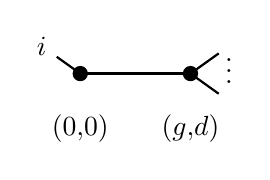
\begin{tikzpicture}[scale=0.7, baseline=-3pt,label distance=0.3cm,thick,
    virtnode/.style={circle,draw,scale=0.5}, 
    nonvirt node/.style={circle,draw,fill=black,scale=0.5} ]
    \node [nonvirt node,label=below:$(0{,}0)$] (A) {};
    \node at (2,0) [nonvirt node,label=below:$(g{,}d)$] (B) {};
    \draw [-] (A) to (B);
    \node at (-.7,.5) (n1) {$i$};
    \draw [-] (A) to (n1);
    \node at (2.7,.5) (m1) {};
    \node at (2.7,-.5) (m2) {};
    \draw [-] (B) to (m1);
    \draw [-] (B) to (m2);    
    \node at (2.7,0.2) (m3) {$\vdots$};
    \end{tikzpicture} 
\to 
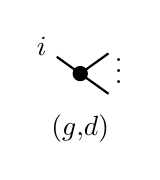
\begin{tikzpicture}[scale=0.7, baseline=-3pt,label distance=0.3cm,thick,
    virtnode/.style={circle,draw,scale=0.5}, 
    nonvirt node/.style={circle,draw,fill=black,scale=0.5} ]
    \node [nonvirt node,label=below:$(g{,}d)$] (A) {};
    \node at (-.7,.5) (n1) {$i$};
    \draw [-] (A) to (n1);
    \node at (.7,.5) (m1) {};
    \node at (.7,-.5) (m2) {};
    \draw [-] (A) to (m1);
    \draw [-] (A) to (m2);    
    \node at (.7,0.2) (m3) {$\vdots$};
    \end{tikzpicture}\ \ .
\]
\end{enumerate}
\end{lemma}
\begin{proof} 
%(1) Straightforward to check. \jocomment{I think (1) is not true, or is it? I would think that $(\sourcemap)^*[\Picabs_{\Gamma_{\delta}}]$ is the union over all $\frak N_{\Gamma_\delta \to \tilde \Gamma_\delta}$ for partial stabilizations $\Gamma_\delta \to \tilde \Gamma_\delta$. But I also think we won't need (1) below.}\textcolor{brown}{Y. Yes, you are completely right. I will remove it.}

\noindent(i) There are two pairs of universal curves with line bundle $(\frak C,\frak L)$ and $(\frak C', \frak L')$
\begin{center}
\begin{tikzcd}
\frak C' \arrow[dr,"\pi'"] \arrow[rr, "f"]
&~
& \frak C \arrow[dl,"\pi"] \\
~
&\frak N_{g,n,d}
&~
\end{tikzcd}
\end{center}
over the stack $\frak{N}_{g,n,d}$ with sections $\sigma_i:\frak N_{g,n,d}\to\frak C$ and $\sigma_i':\frak N_{g,n,d}\to \frak C'$. Because $f_*[\frak C'] = [\frak C]$, we have
\[
\targetmap^*\eta = \pi_*(c_1(\frak L)^2) = \pi_*(c_1(\frak L)^2f_*[\frak C']) = \pi'_*(c_1(f^*\frak L)^2) = (\sourcemap)^*\eta\, .
\]

\noindent (ii) Let $D'_0$ be the divisor
\[
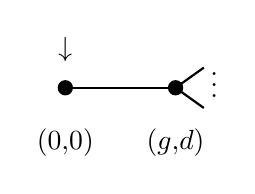
\begin{tikzpicture}[scale=0.7, baseline=-3pt,label distance=0.3cm,thick,
    virtnode/.style={circle,draw,scale=0.5}, 
    nonvirt node/.style={circle,draw,fill=black,scale=0.5} ]
    \node [nonvirt node,label=below:$(0{,}0)$] (A) {};
    \node at (2,0) [nonvirt node,label=below:$(g{,}d)$] (B) {};
    \draw [-] (A) to (B);
    %\node at (-.7,.5) (n1) {$i$};
    %\draw [-] (A) to (n1);
    \node at (0,.7) (n2) {$\downarrow$};
    \node at (2.7,.5) (m1) {};
    \node at (2.7,-.5) (m2) {};
    \draw [-] (B) to (m1);
    \draw [-] (B) to (m2);    
    \node at (2.7,0.2) (m3) {$\vdots$};
    \end{tikzpicture} 
\to 
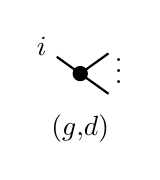
\begin{tikzpicture}[scale=0.7, baseline=-3pt,label distance=0.3cm,thick,
    virtnode/.style={circle,draw,scale=0.5}, 
    nonvirt node/.style={circle,draw,fill=black,scale=0.5} ]
    \node [nonvirt node,label=below:$(g{,}d)$] (A) {};
    \node at (-.7,.5) (n1) {$i$};
    \draw [-] (A) to (n1);
    \node at (.7,.5) (m1) {};
    \node at (.7,-.5) (m2) {};
    \draw [-] (A) to (m1);
    \draw [-] (A) to (m2);    
    \node at (.7,0.2) (m3) {$\vdots$};
    \end{tikzpicture}
\]
% \[
% \begin{tikzpicture}[scale=0.7, baseline=-3pt,label distance=0.3cm,thick,
%     virtnode/.style={circle,draw,scale=0.5}, 
%     nonvirt node/.style={circle,draw,fill=black,scale=0.5} ]
%     \node [nonvirt node,label=below:$(0{,}0)$] (A) {};
%     \node at (2,0) [nonvirt node,label=below:$(g{,}d)$] (B) {};
%     \node at (2,.7) (n1) { $\downarrow$};
%     \draw [-] (A) to (B);
%     \node at (2.7,.5) (m1) {};
%     \node at (2.7,-.5) (m2) {};
%     \draw [-] (B) to (m1);
%     \draw [-] (B) to (m2);    
%     \node at (2.7,0.2) (m3) {$\vdots$};
%     \end{tikzpicture} 
% \]
in $\frak C'$, and let $D'_i$ be the divisor
\[
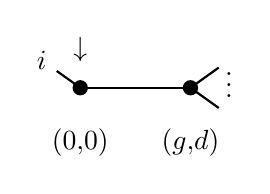
\begin{tikzpicture}[scale=0.7, baseline=-3pt,label distance=0.3cm,thick,
    virtnode/.style={circle,draw,scale=0.5}, 
    nonvirt node/.style={circle,draw,fill=black,scale=0.5} ]
    \node [nonvirt node,label=below:$(0{,}0)$] (A) {};
    \node at (2,0) [nonvirt node,label=below:$(g{,}d)$] (B) {};
    \draw [-] (A) to (B);
    \node at (-.7,.5) (n1) {$i$};
    \draw [-] (A) to (n1);
    \node at (0,.7) (n2) {$\downarrow$};
    \node at (2.7,.5) (m1) {};
    \node at (2.7,-.5) (m2) {};
    \draw [-] (B) to (m1);
    \draw [-] (B) to (m2);    
    \node at (2.7,0.2) (m3) {$\vdots$};
    \end{tikzpicture} 
\to 
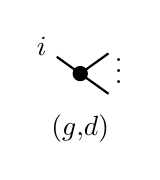
\begin{tikzpicture}[scale=0.7, baseline=-3pt,label distance=0.3cm,thick,
    virtnode/.style={circle,draw,scale=0.5}, 
    nonvirt node/.style={circle,draw,fill=black,scale=0.5} ]
    \node [nonvirt node,label=below:$(g{,}d)$] (A) {};
    \node at (-.7,.5) (n1) {$i$};
    \draw [-] (A) to (n1);
    \node at (.7,.5) (m1) {};
    \node at (.7,-.5) (m2) {};
    \draw [-] (A) to (m1);
    \draw [-] (A) to (m2);    
    \node at (.7,0.2) (m3) {$\vdots$};
    \end{tikzpicture}
\]
% \[
% \begin{tikzpicture}[scale=0.7, baseline=-3pt,label distance=0.3cm,thick,
%     virtnode/.style={circle,draw,scale=0.5}, 
%     nonvirt node/.style={circle,draw,fill=black,scale=0.5} ]
%     \node [nonvirt node,label=below:$(0{,}0)$] (A) {};
%     \node at (2,0) [nonvirt node,label=below:$(g{,}d)$] (B) {};
%     \draw [-] (A) to (B);
%     \node at (-.7,.5) (n1) {$i$};
%     \draw [-] (A) to (n1);
%     \node at (2,.7) (n2) {$\downarrow$};
%     \node at (2.7,.5) (m1) {};
%     \node at (2.7,-.5) (m2) {};
%     \draw [-] (B) to (m1);
%     \draw [-] (B) to (m2);    
%     \node at (2.7,0.2) (m3) {$\vdots$};
%     \end{tikzpicture}
% \]
in $\frak C'$. Here, the arrows pointing to the vertices with genus and degree $0$ indicate which component of the universal curve over the corresponding boundary divisor in $\frak N_{g,n,d}$ we take. The divisors $D_0', D_1', \ldots, D_n'$ are precisely the divisorial loci in $\frak C'$ which are contracted by the map $f: \frak C' \to \frak C$.
Then 
\[
\targetmap^*\psi_i = c_1(\sigma_i^*\omega_\pi)= ({\sigma}_i')^*c_1(f^*\omega_\pi) = ({\sigma}_i')^* c_1(\omega_{\pi'}(-D'_0-\sum_{i=1}^n D'_i)) = (\sourcemap)^*\psi_i - D_i\, , 
\] 
where the sections are denoted by $\sigma_i$.
\end{proof}


For the morphism $\sourcemap$, form the  fibre diagram 
\begin{equation} \label{eqn:frakNdiagrampprime}
\source{pixtons-formula-abel-jacobi-picard-stack}
\begin{tikzcd}
  \Picabs'_{\Gamma_{\delta}}\arrow[d]\arrow[r,"J'_{\Gamma_{\delta}}"] & \frak N\arrow[d,"\sourcemap"]\\
\Picabs_{\Gamma_{\delta}}\ar[r,"j_{\Gamma_{\delta}}"] & \Picabs_{g,0,0}. 
\end{tikzcd}
\end{equation}
By definition, the fibre product $\Picabs'_{\Gamma_{\delta}}$ parametrizes data
\[(C_v')_{v \in \V(\Gamma)}\, , \,\, \ca L'/C'=\sqcup_v C_v'\, , \,\, f: C' \to C\, , \,\, \ca L/C\, , \,\, f^* \ca L \xrightarrow{\sim} \ca L'\]
which simplifies to
\[(C_v')_{v \in \V(\Gamma)}\, , \,\, f: \sqcup_v C_v' = C' \to C\, , \,\, \ca L/C\, .\]
On the other hand, the stack $\frak N_{\Gamma_\delta}'$   parametrizes
\[
(C_v)_{v\in \V(\Gamma)}\, , \,\, \ca L/C\, , \,\, (f_v:C'_v\to C_v)_{v\in \V(\Gamma)}\, .
\]
There is a subtle difference here. For $\Picabs'_{\Gamma_{\delta}}$, the map $f$ is allowed to contract entire components $C_v'$ to points, whereas in the second case the target $C_v$ is always still 1-dimensional.


Our next step is to show 
\begin{equation} \label{eqn:Picabsprimeiso}
\source{pixtons-formula-abel-jacobi-picard-stack}
\Picabs'_{\Gamma_{\delta}} \cong \sqcup_{\Gamma_{\delta}\to \tilde{\Gamma}_{\delta}} \frak N_{\Gamma_{\delta}\to \tilde{\Gamma}_{\delta}}\, .\end{equation}
More precisely,
the connected components of $\Picabs'_{\Gamma_{\delta}}$ are in bijective correspondence to partial stabilizations $$\Gamma_{\delta}\to\tilde{\Gamma}_{\delta}\, .$$
We will prove, given a vertex $v \in \V(\Gamma)$ which can be contracted (with $g(v)=0$, $n(v) \leq 2$, $\delta(v)=0$), that
the locus of points in $\Picabs'_{\Gamma_{\delta}}$ where $f: C' \to C$ contracts $C_v'$ is open and closed.

For a vertex $v$ with $n(v)=2$, the universal curve $\frak C_v' \to \Picabs'_{\Gamma_{\delta}}$ has two sections (corresponding to the half-edges at $v$), and the locus where $C_v'$ is contracted equals the locus where the sections coincide, which is closed since $\frak C_v' \to \Picabs'_{\Gamma_{\delta}}$ is separated. 

To show closedness of the locus where $C_v'$ is \emph{not} contracted, assume we have a family 
\[(C_{v,S}')_{v \in \V(\Gamma)}\, , \,\, f: \sqcup_v C_{v,S}' = C_S' \to C_S\, , \,\, \ca L/C_S\, \]
of $\Picabs'_{\Gamma_{\delta}}$ over the spectrum $S$ of a strictly henselian DVR such that the fibre $C'_{v,\eta}$ of $C'_{v,S}$ over the generic point $\eta$ of $S$ is not contracted by $f$. We want to show that then also the fibre $C'_{v,L}$ over the closed point $L$ of $S$ is not contracted. By assumption,  $C'_{v,\eta}$ maps to a union $C_{v,\eta}$ of components of the fibre $C_\eta$ of $C_S$ over $\eta$. Then $C_{v,\eta}$ specializes to a union $C_{v,L}$ of components of $C_L$. Since $f$ is proper, $f$ maps the closure $C'_{v,S}$ of $C'_{v,\eta}$ to the closure of its image $C_{v,\eta}$. Since $C_{v,L}$ is still positive-dimensional, the curve $C'_{v,L}$ is indeed not contracted. For related arguments, see the proof of \cite[Proposition 2.2]{Kresch2013Flattening-stra}. 

% Younghan and I were stuck on showing that its complement is closed. This should be implied if we show that for a DVR $R$ (with closed point $L$ and open point $\eta$) and an $R$-point of $\Picabs'_{\Gamma_{\delta}}$ such that $C_{v,\eta}'$ is not contracted under $f$, then also $C_{v,L}'$ is not contracted. This seems very plausible: we can assume that the image $C_{v,\eta}$ of $C_{v,\eta}'$ under $f$ is a component of the flat map $C_\eta \to \on{Spec}(R)$ and it seems like its closure should not be a allowed to have a single point (the image of the contracted $C_{v,L}'$) as its specialization over $L$. Someone with basic knowledge of algebraic geometry to the rescue??

For a vertex $v$ with $n(v)=1$, the universal curve $\frak C_v' \to \Picabs'_{\Gamma_{\delta}}$ has a single section $\sigma_h$. On the one hand, the locus where $C_v'$ is contracted is exactly the locus where $f : \frak C' \to \frak C$ maps $\sigma_h$ to the smooth locus of $\frak C \to \Picabs'_{\Gamma_{\delta}}$, thus it is open. On the other hand, it is also the preimage under $\sigma_h$ of the exceptional locus of $\frak C' \to \frak C$, and thus closed.

We have proven that the connected components of $\Picabs'_{\Gamma_{\delta}}$ are in bijective correspondence to partial stabilizations $\Gamma_{\delta}\to\tilde{\Gamma}_{\delta}$. But a point 
\[(C_v')_{v \in \V(\Gamma)}\, , \,\, f: \sqcup_v C_v' = C' \to C\, , \,\, \ca L/C\]
on the corresponding component is equivalent to the data of any collection of curves $C_v'$ for $v' \in \V(\Gamma) \setminus \V(\tilde \Gamma)$, which are contracted by $f$, together with a point
\[(C_v')_{v \in \V(\tilde \Gamma)}\, , \,\, f: (C_v' \to C_v)\, , \,\, \ca L/C = \sqcup_{v \in V(\tilde \Gamma)} C_v\]
of $\frak N'_{\Tilde{\Gamma}_{\delta}}$. Hence, we have a isomorphism
\[\frak N_{\Gamma_{\delta}\to \tilde{\Gamma}_{\delta}} \cong \frak N'_{\Tilde{\Gamma}_{\delta}}\times \prod_{v\in \V(\Gamma)\setminus \V(\Tilde{\Gamma})} \frak M_{0,\n(v)}\, ,\]
where, in the last expression, $n(v)$ is necessarily $1$ or $2$.

% \{Maybe we want something like the following (haven't completely understood the above though). 

% Let $S$ be spec of a strictly hensellian DVR, and $f\colon C'\to C$ a map of prestable curves over $S$. Let $C_v$ be a connected component of the normalisation of $C_\eta$, with closure $\bar C_v$. Assume that $f$ is not constant on $C_v$. Then $f$ is not constant on the fibre $\bar C_v \times_S s$ (it may contract some components, but not all). 

% Proof. 
% $f$ is proper, so its image is closed, hence contains (in fact, equals) the closure of $f(C_v)$. But this is the closure of an irreducible component of a prestable curve, so its closed fibre has positive dimension. \qed
% }

For each partial stabilisation $\Gamma_{\delta}\to \tilde{\Gamma}_{\delta}$, we denote by $$J_{\Gamma_{\delta}\to\tilde{\Gamma}_{\delta}}: \frak N_{\Gamma_{\delta}\to\tilde{\Gamma}_{\delta}}\to \frak N$$ the restriction of $J'_{\Gamma_{\delta}}$ to $\frak N_{\Gamma_{\delta}\to \tilde{\Gamma}_{\delta}}$.  
\begin{lemma}
\source{pixtons-formula-abel-jacobi-picard-stack}
\notready\label{lem:N_invariance_P}
\source{pixtons-formula-abel-jacobi-picard-stack}
We have $\targetmap^* \P_{g}^\bullet = (\sourcemap)^* \P_g^\bullet
\, \in\, \prod_{c=0}^\infty {\mathsf{CH}}^c_{\mathsf{op}}(\frak N)$
for all $c \geq 0$. 
\end{lemma}
\begin{proof} 
We will use  formula \eqref{eqn:P_gformula2}
for $\P_g^\bullet$. By \cref{lem:pullback_comparison}, the terms $\exp(- \eta/2)$ have identical pullback under $\targetmap$ and $\sourcemap$. We can therefore
focus on the sum over graphs and weighting mod $r$. 

We start with a few remarks about the combinatorial factors in $\P_g^\bullet$ which will arise in the proof. Let $\Gamma_{\delta}\to\tilde{\Gamma}_{\delta}$ be a partial stabilization, then the Betti numbers agree,
$$h^1(\Gamma_\delta) = h^1(\tilde \Gamma_\delta)\, .$$
Given $r$, the map $W_{\Gamma_\delta,r} \to W_{\tilde \Gamma_\delta, r}$ of admissible weightings mod $r$ (induced by the inclusion $H(\tilde \Gamma) \to H(\Gamma)$ of half-edge sets) is a bijection. 

Moreover, if the map $\Gamma_{\delta}\to\tilde{\Gamma}_{\delta}$ only contracts components with $$(\g(v),\n(v),\delta(v))=(0,2,0)\,,$$ there is a canonical isomorphism $\Aut(\Gamma_\delta) \cong \Aut(\tilde \Gamma_\delta)$. On the other hand, in the formula for $\P_g^\bullet$, every term such that $\Gamma_\delta$ has a vertex with $$(\g(v), \n(v), \delta(v))=(0,1,0)$$ necessarily vanishes. Indeed, the half-edge $h$ at this vertex must have $w(h)=0$ such that the corresponding edge term vanishes. 

To keep the notation concise, we write $\Phi_{a}$ for the power-series 
\begin{align*} 
\Phi_{a}(x)&= \frac{1-\exp({-\frac{a}{2}}x)}{x}\\ &= \sum_{m=0}^\infty (-1)^m (\frac{a}{2})^{m+1} \frac{1}{(m+1)!}x^m = \frac{a}{2} - \frac{a^2}{8} x + \ldots 
\end{align*}
appearing in the edge terms of $\P_g^\bullet$. Moreover, given a graph $\tilde \Gamma_\delta$ with a half-edge $h$ incident to a vertex $v$, denote by $\psi_h, \psi_h'$ the classes on $\frak N'_{\tilde \Gamma_\delta}$ pulled back from $\frak N_{\g(v),\n(v),\delta(v)}$ in the diagram \eqref{eqn:frakNdiagramp}. Similarly, given a partial stabilization $\Gamma_\delta \to \tilde \Gamma_\delta$, the space $\frak N_{\Gamma_\delta \to \tilde \Gamma_\delta}$ contains $\frak N'_{\tilde \Gamma_\delta}$ as a factor, hence the notation also makes sense on $\frak N_{\Gamma_\delta \to \tilde \Gamma_\delta}$ (provided $h$ is a half-edge of $\tilde \Gamma_\delta$).

Let us first compute the pullback of the graph sum in $\P_g^{\bullet,r}$ via $\sourcemap : \frak N \to \Picabs_{g,0,0}$. Using the diagram \eqref{eqn:frakNdiagrampprime} and the decomposition \eqref{eqn:Picabsprimeiso}, we see
\begin{align} 
&(\sourcemap)^* \sum_{\Gamma_\delta, w}
\frac{r^{-h^1( \Gamma_\delta)}}{|\Aut(\Gamma_\delta)| }
\;
j_{\Gamma_\delta*}\Bigg[
\prod_{e=(h,h')\in \E(\Gamma_\delta)}
\Phi_{w(h)w(h')}(\psi_h + \psi_{h'}) \Bigg] \nonumber\\
=&\sum_{\Gamma_\delta \to \tilde \Gamma_\delta, w} \label{eqn:pprimepullb}
\source{pixtons-formula-abel-jacobi-picard-stack}
\frac{r^{-h^1( \Gamma_\delta)}}{|\Aut(\Gamma_\delta)| }
\;
J_{\Gamma_\delta \to \tilde \Gamma_\delta*}\Bigg[
\prod_{e=(h,h')\in \E(\Gamma_\delta)}
\Phi_{w(h)w(h')}(\psi'_h + \psi'_{h'}) \Bigg]\, .
\end{align}
In the second line, the sum is over all partial stabilizations $\Gamma_\delta \to \tilde \Gamma_\delta$.

Second, we compute the pullback of the graph sum in $\P_g^{\bullet,r}$ via $\targetmap : \frak N \to \Picabs_{g,0,0}$
\begin{align} 
&\targetmap^* \sum_{\tilde \Gamma_\delta, w}
\frac{r^{-h^1(\tilde  \Gamma_\delta)}}{|\Aut(\tilde \Gamma_\delta)| }
\;
j_{\tilde \Gamma_\delta*}\Bigg[
\prod_{e=(h,h')\in \E(\tilde \Gamma_\delta)}
\Phi_{w(h)w(h')}(\psi_h + \psi_{h'}) \Bigg]\nonumber \\
=&\sum_{\tilde \Gamma_\delta, w}\label{eqn:ppullb}
\source{pixtons-formula-abel-jacobi-picard-stack}
\frac{r^{-h^1(\tilde \Gamma_\delta)}}{|\Aut(\tilde \Gamma_\delta)| }
\;
\widehat J_{\tilde \Gamma_\delta*}\Bigg[
\prod_{e=(h,h')\in \E(\tilde \Gamma_\delta)}
\Phi_{w(h)w(h')}(\psi_h + \psi_{h'}) \Bigg]\, .
\end{align}
We use here the right fibre diagram in \eqref{eqn:frakNdiagramp} together with the fact that $G$ is proper, representable, and birational.  So by Proposition \ref{prop:invarianceproperbirat},
the pushforward of fundamental classes under $J_{\tilde \Gamma_\delta}$ and $\widehat J_{\tilde \Gamma_\delta}$ agree.

To compare to the formula for the pullback under $\sourcemap$, we use 
$$\psi_h + \psi_{h'} = \psi_h' - D_h + \psi_{h'}'- D_{h'}$$ on $\frak N'_{\tilde \Gamma_\delta}$ by \cref{lem:pullback_comparison}.
%By \cref{lem:pullback_comparison}, it is enough to show that the pullback of each edge term along $\targetmap$ and $\sourcemap$ coincide. For simplicity, we introduce a function $\Phi_{e,w}(x)= \frac{1-\exp({-\frac{w(h)w(h')}{2}}x)}{x}$ for each edge $e=(h,h')$. 
The next step of the proof is to use the self-intersection formula for $D_h, D_{h'}$ (similar to the formula described in \cite[Appendix A]{GraberPandharipande}) to expand the edge term
\[\Phi_{w\,w'}(\psi_h' - D_h + \psi_{h'}'- D_{h'}) = \sum_{m=0}^\infty (-1)^m (\frac{w\,w'}{2})^{m+1} \frac{1}{(m+1)!}(\psi_h' - D_h + \psi_{h'}'- D_{h'})^m.\] For example, $(D_h)^2$ is equal to
\begin{equation*}
-
    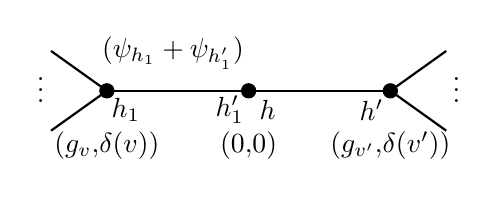
\begin{tikzpicture}[scale=1.2, baseline=-3pt,label distance=0.3cm,thick,
    virtnode/.style={circle,draw,scale=0.5}, 
    nonvirt node/.style={circle,draw,fill=black,scale=0.5} ]
    \node at (0,0) [nonvirt node,label=below:$(g_{v}{,}\delta(v))$] (A) {};
    \node at (1.5,0) [nonvirt node,label=below:$(0{,}0)$] (C) {};    
    \node at (3,0) [nonvirt node,label=below:$(g_{v'}{,}\delta(v'))$] (B) {};
    \node at (.2,-.2) {$h_1$};
    \node at (1.3,-.2) {$h'_1$}; 
    \node at (1.7,-.2) {$h$};
    \node at (2.8,-.2) {$h'$};
    \draw [-] (A) to (C);
    \draw [-] (B) to (C);
    \node at (.7,.4) {$(\psi_{h_1}+\psi_{h'_1})$};
    \node at (3.7,.5) (m1) {};
    \node at (3.7,-.5) (m2) {};
    \draw [-] (B) to (m1);
    \draw [-] (B) to (m2);    
    \node at (3.7,0.1) (m3) {$\vdots$};
    \node at (-0.7,.5) (n1) {};
    \node at (-0.7,-.5) (n2) {};
    \draw [-] (A) to (n1);
    \draw [-] (A) to (n2);    
    \node at (-.7,0.1) (n3) {$\vdots$};    
    \end{tikzpicture}
+ \,2
    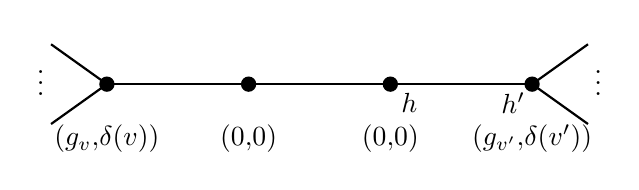
\begin{tikzpicture}[scale=1.2, baseline=-3pt,label distance=0.3cm,thick,
    virtnode/.style={circle,draw,scale=0.5}, 
    nonvirt node/.style={circle,draw,fill=black,scale=0.5} ]
    \node at (0,0) [nonvirt node,label=below:$(g_{v}{,}\delta(v))$] (A) {};
    \node at (1.5,0) [nonvirt node,label=below:$(0{,}0)$] (C) {};   
    \node at (3,0) [nonvirt node,label=below:$(0{,}0)$] (D) {}; 
    \node at (4.5,0) [nonvirt node,label=below:$(g_{v'}{,}\delta(v'))$] (B) {};
    \node at (3.2,-.2) {$h$};
    \node at (4.3,-.2) {$h'$};
    \draw [-] (A) to (C);
    \draw [-] (C) to (D);
    \draw [-] (D) to (B);
    \node at (5.2,.5) (m1) {};
    \node at (5.2,-.5) (m2) {};
    \draw [-] (B) to (m1);
    \draw [-] (B) to (m2);    
    \node at (5.2,0.1) (m3) {$\vdots$};
    \node at (-0.7,.5) (n1) {};
    \node at (-0.7,-.5) (n2) {};
    \draw [-] (A) to (n1);
    \draw [-] (A) to (n2);    
    \node at (-.7,0.1) (n3) {$\vdots$};    
    \end{tikzpicture}
\end{equation*}
and similarly for $(D_{h'})^2$.

The result will be a linear combination of terms
\begin{equation}
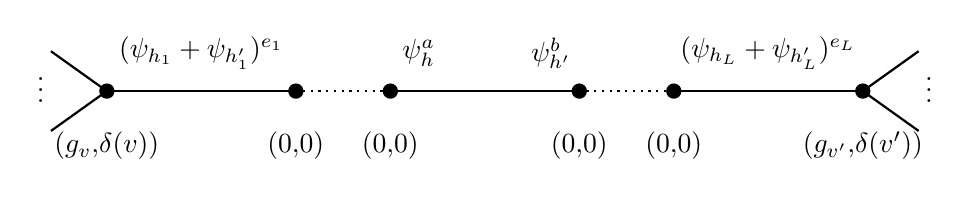
\begin{tikzpicture}[scale=1.2, baseline=-3pt,label distance=0.3cm,thick,
    virtnode/.style={circle,draw,scale=0.5}, 
    nonvirt node/.style={circle,draw,fill=black,scale=0.5} ]
    \node at (-6,0) [nonvirt node,label=below:$(g_{v}{,}\delta(v))$] (F) {};
    \node at (-4,0) [nonvirt node,label=below:$(0{,}0)$] (E) {};
    \node at (-3,0) [nonvirt node,label=below:$(0{,}0)$] (D) {};
    \node at (-1,0) [nonvirt node,label=below:$(0{,}0)$] (C) {};
    \node [nonvirt node,label=below:$(0{,}0)$] (A) {};
    \node at (2,0) [nonvirt node,label=below:$(g_{v'}{,}\delta(v'))$] (B) {};
    \draw [-] (A) to (B);
    \draw [-, dotted] (C) to (A);
    \draw [-] (D) to (C);
    \draw [-, dotted] (E) to (D);
    \draw [-] (F) to (E);
    \node at (1,.4) {$(\psi_{h_L}+\psi_{h'_L})^{e_L}$};
    \node at (-5,.4) {$(\psi_{h_1}+\psi_{h'_1})^{e_1}$};
    \node at (-2.7,.4) {$\psi_h^a$};
    \node at (-1.3,.4) {$\psi_{h'}^b$};
    %\node at (-.7,.5) (n1) {$i$};
    %\draw [-] (A) to (n1);
    %\node at (0,.7) (n2) {$\downarrow$};
    \node at (2.7,.5) (m1) {};
    \node at (2.7,-.5) (m2) {};
    \draw [-] (B) to (m1);
    \draw [-] (B) to (m2);    
    \node at (2.7,0.1) (m3) {$\vdots$};
    \node at (-6.7,.5) (n1) {};
    \node at (-6.7,-.5) (n2) {};
    \draw [-] (F) to (n1);
    \draw [-] (F) to (n2);    
    \node at (-6.7,0.1) (n3) {$\vdots$};    
    \end{tikzpicture}
\end{equation}
where the edge $(h,h')$ is at position $\ell$ in the above chain ($1 \leq \ell \leq L$). The total degree of this term (before the pushforward by $\widehat J_{\tilde \Gamma_\delta}$) is
\[m = \sum_{j \neq \ell} (e_j+1) + a + b\, .\]
The total coefficient of this particular term in $\Phi_{w\,w'}(\psi_h' - D_h + \psi_{h'}'- D_{h'})$ is then
\[
%\mathrm{Coeff} = 
\underbrace{(-1)^m (\frac{w\,w'}{2})^{m+1} \frac{1}{(m+1)!}}_{\text{coeff in $\Phi_{w\,w'}$}}\cdot \binom{m}{e_1+1, \ldots, a,b,\ldots, e_L+1} \underbrace{(-1)^{L-1}}_{\substack{\text{excess intersection}\\\text{of $-D_h, -D_{h'}$}}} % \underbrace{(-1)^{\sum_{j \neq i} e_j+1}}_{\text{sign from $-D_h, -D_{h'}$}} \cdot \underbrace{(-1)^{\sum_{j \neq i} e_j}}_{\text{excess intersection}},
\]
where the multinomial coefficient comes from the expansion of $$(\psi_h' - D_h + \psi_{h'}'- D_{h'})^m\, .$$
Writing $e_\ell=a+b$, we can simplify to obtain
\[
%\mathrm{Coeff} = 
\frac{1}{m+1}
\left(\prod_{j=1}^L (-1)^{e_j} (\frac{w\,w'}{2})^{e_j+1} \frac{1}{(e_j+1)!} \right) \binom{e_\ell}{a} (e_\ell+1)\, .
\]
Summing over all choices $a+b=e_\ell$ for fixed $e_\ell$, the coefficient of the term
\begin{equation}
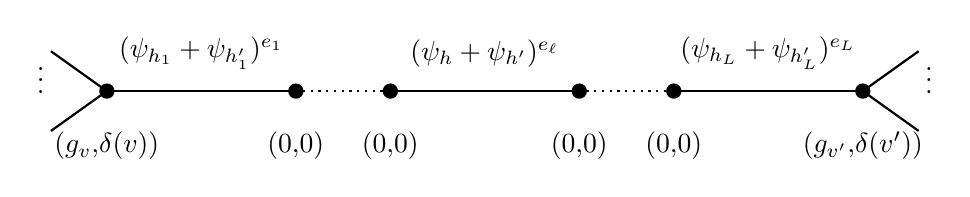
\begin{tikzpicture}[scale=1.2, baseline=-3pt,label distance=0.3cm,thick,
    virtnode/.style={circle,draw,scale=0.5}, 
    nonvirt node/.style={circle,draw,fill=black,scale=0.5} ]
    \node at (-6,0) [nonvirt node,label=below:$(g_{v}{,}\delta(v))$] (F) {};
    \node at (-4,0) [nonvirt node,label=below:$(0{,}0)$] (E) {};
    \node at (-3,0) [nonvirt node,label=below:$(0{,}0)$] (D) {};
    \node at (-1,0) [nonvirt node,label=below:$(0{,}0)$] (C) {};
    \node [nonvirt node,label=below:$(0{,}0)$] (A) {};
    \node at (2,0) [nonvirt node,label=below:$(g_{v'}{,}\delta(v'))$] (B) {};
    \draw [-] (A) to (B);
    \draw [-, dotted] (C) to (A);
    \draw [-] (D) to (C);
    \draw [-, dotted] (E) to (D);
    \draw [-] (F) to (E);
    \node at (1,.4) {$(\psi_{h_L}+\psi_{h'_L})^{e_L}$};
    \node at (-5,.4) {$(\psi_{h_1}+\psi_{h'_1})^{e_1}$};
    \node at (-2,.4) {$(\psi_{h}+\psi_{h'})^{e_\ell}$};
    %\node at (-.7,.5) (n1) {$i$};
    %\draw [-] (A) to (n1);
    %\node at (0,.7) (n2) {$\downarrow$};
    \node at (2.7,.5) (m1) {};
    \node at (2.7,-.5) (m2) {};
    \draw [-] (B) to (m1);
    \draw [-] (B) to (m2);    
    \node at (2.7,0.2) (m3) {$\vdots$};
    \node at (-6.7,.5) (n1) {};
    \node at (-6.7,-.5) (n2) {};
    \draw [-] (F) to (n1);
    \draw [-] (F) to (n2);    
    \node at (-6.7,0.2) (n3) {$\vdots$};    
    \end{tikzpicture}
\end{equation}
is exactly equal to
\[
%\mathrm{Coeff} = 
\frac{e_\ell +1}{m+1}
\left(\prod_{j=1}^L (-1)^{e_j} (\frac{w\,w'}{2})^{e_j+1} \frac{1}{(e_j+1)!} \right).
\]
Pushing forward by $\widehat J_{\tilde \Gamma_\delta}$, we forget where in the chain above the edge $(h,h')$ has been. Summing over the $L$ possible positions and using $m+1 = \sum_{\ell=1}^L (e_\ell +1)$, we obtain the coefficient
\[\prod_{j=1}^L \underbrace{(-1)^{e_j} (\frac{w\,w'}{2})^{e_j+1} \frac{1}{(e_j+1)!}}_{\text{coefficient of $x^{e_j}$ in $\Phi_{w\,w'}(x)$}}\, .\]
From the above discussion, we see that \eqref{eqn:ppullb} equals
\[\sum_{\Gamma_\delta \to \tilde \Gamma_\delta, w}
\frac{r^{-h^1( \tilde \Gamma_\delta)}}{|\Aut(\tilde \Gamma_\delta)| }
\;
J_{\Gamma_\delta \to \tilde \Gamma_\delta*}\Bigg[
\prod_{e=(h,h')\in \E(\Gamma_\delta)}
\Phi_{w(h)w'(h)}(\psi'_h + \psi'_{h'}) \Bigg]\, .\]
%Here, a priori 
The sum goes over stabilizations $\Gamma_\delta \to \tilde \Gamma_\delta$ contracting chains of curves with $(g,n,d)=(0,2,0)$.
By the previous remarks concerning the combinatorial factors, we have
\[h^1( \tilde \Gamma_\delta) = h^1(\Gamma_\delta)\, , \ \ \ |\Aut(\tilde \Gamma_\delta)| = |\Aut(\Gamma_\delta)|\, . \]
The sum does not change if we allow arbitrary stabilizations $\Gamma_\delta \to \tilde \Gamma_\delta$, since for $\Gamma_\delta$ having a vertex with $(g,n,d)=(0,1,0)$, the summand automatically vanishes. Thus the sum above equals the term computed in \eqref{eqn:pprimepullb}. 
% We first prove the case when $\E(\Gamma)=\{e=(h,h')\}$ with weight $w$. For each partial stabilization $\hat{\Gamma}_{\delta}\to \Gamma_{\delta}$, there exists a unique weighting $\hat{w}$ on $\hat{\Gamma}_{\delta}$ with $\hat{w}(h)=w(h)$ and $\hat{w}(h')=w(h')$. Then 
% \begin{equation*}
% \begin{split}
% \targetmap^*j_{\Gamma_{\delta}*}\Phi_{e,w}(\psi_h+\psi_{h'}) &= J_{\Gamma_{\delta}*}\targetmap^*\Phi_{e,w}(\psi_h+\psi_{h'}) \\
% &=J_{\Gamma_{\delta}*}\Phi_{e,w}((\sourcemap)^*(\psi_h+\psi_{h'})-D_h-D_{h'})\\
% &= ... \\
% &=\sum_{\hat{\Gamma}_{\delta}\to\Gamma_{\delta}}J'_{\hat{\Gamma}_{\delta}\to\Gamma_{\delta}*}\prod_{e\in\E(\hat{\Gamma})}\Phi_{e,\hat{w}}((\sourcemap)^*(\psi_h+\psi_{h'}))\\
% &=\sum_{\hat{\Gamma}_{\delta}\to\Gamma_{\delta}}(\sourcemap)^* J_{\hat{\Gamma}_{\delta}\to\Gamma_{\delta}*}\prod_{e\in\E(\hat{\Gamma})}\Phi_{e,\hat{w}}(\psi_h+\psi_{h'})\\
% &=\sum_{\hat{\Gamma}_{\delta}}(\sourcemap)^*j_{\hat{\Gamma}_{\delta}*}\prod_{e\in\E(\hat{\Gamma})}\Phi_{e,\hat{w}}(\psi_h+\psi_{h'})
% \end{split}
% \end{equation*}
% where $\hat{\Gamma}_{\delta}\to\Gamma_{\delta}$ is all partial stabilization. The third equality comes from the excess intersection formula of $(D_h)^k$. For general graph $\Gamma_{\delta}$, we can use the formula above at each edge. 
\end{proof}
%Now we show \cref{eq:pullback_pixton}, continuing in the notation we just set up. Choose a vector of integers $A=(\bd 0, a_{n+1},\cdots,a_{n+m})\in \mathbb{Z}^{n+m}$ such that $\ca L'(AP)$ is relatively very ample. Let $p\colon U_{l}'\to B'$ be the scheme over $B'$ constructed in \cref{sec:very_ample}.  Consider the following diagram
%\begin{equation}
% \begin{tikzcd}
%  U'_l \arrow[r, "\phi_{\ca L'(AP)}"]\arrow[d, "p"]& \overline{\mathcal{M}}_{g,n+m}(X,\beta) \arrow[d, "\phi_{f^*\ca O(1)\otimes(-AP)}"] \\
%  B' \arrow[r, "\ca \phi_{\ca L'}"]\arrow[d, "h"]\arrow[dr, "\phi_{\ca L'}"] & \Picabs_{g,n+m} \arrow[d]\\
%  B \arrow[r, "\phi_{\ca L}"]  & \Picabs_{g,n}.
%\end{tikzcd}
%\end{equation}
%where the lower left corner is not commutative. Since the pull back along $p$ is injective, it is enough to prove \cref{eq:pullback_pixton} on $U_{l}'$. In principle, 
%$\phi_{\ca L}^*\P_{g,\bd 0,0}^g(h \circ p)$ has all contributions from some chains of $\bb P^1$s which was inserted. After restricting to $\Picabs'$, contributions from $\bb P^1$ chains where line bundle has degree $0$ vanishes. 
%On the other hand, $\phi_{\ca L'(AP)} : U_{l}'\to \Picabs_{g,n+m}$ factors through $\overline{\mathcal{M}}_{g,n+m}(X,\beta)$, so on the unstable locus, the degree of the line bundle should be positive. Therefore we do not have contributions from $\PP^1$ chains with degree $0$. 
%=========

%I think the advantage for the proof of invariance under $\Phi$ is that it plays out purely on $\Picabs_{g,n,d}$ and not some strange family parametrized by $B$. For the vertex term $\exp(- \eta/2)$ this will be a standard computation involving the fact that the map $\frak C' \to \frak C$ is birational, thus fundamental class pushes forward to fundamental class. For the sum over graphs, I think there will be natural diagrams
%\[
%\begin{tikzcd}
%\prod_{v \in \V(\Gamma)} \Picabs_{g(v),n(v),\delta(v)} \arrow[d,"\prod_v \Phi_i"] &\Picabs_{\Gamma_{\delta}} \arrow[l] \arrow[r] \arrow[d] & \Picabs_{g,n,0} \arrow[d,"\Phi"]\\
%\prod_{v \in \V(\Gamma)} \Picabs_{g(v),n(v),\delta(v)} &\Picabs_{\Gamma_{\delta}} \arrow[l]\arrow[r] & \Picabs_{g,n,0}
%\end{tikzcd}
%\]
%for $\Gamma_\delta$ not containing a vertex of type $(g,n,d)=(0,0,0)$ (otherwise the fibre product is a bit strange - the generic point has no preimage, but if the $(0,0,0)$-curve degenerates into a $(0,0,a)$ and a $(0,0,-a)$-curve, then it can suddenly have preimages ... to think about). The right square is cartesian (maybe the left too). 

%Are these ingredients enough to show the invariance? I think the terms $\psi_h + \psi_{h'}$ will pull back to themselves \emph{plus} a contribution from inserting an unstable $(g,n,d)=(0,0,0)$-bubble inside the half-edge, and this turns out to be compatible with Pixton's formula?




%, because in the situation of invariance \invnrIV{} we essentially say that we are given a $\ca S$-point of $\ca N$ and then show an equality of operational classes on $\ca S$ pulled back from $\Picabs_{g,0,0}$ via $p,\sourcemap$.
%\{This I completely agree with, and it gives a good perspective on Inv IV. }

%But my hope would be that $\ca N$ exists and that one can do tautological computations on it. Also, I am guessing that the pullbacks of $\aj : \cat{Div}_g \to \Picabs_{g,0,0}$ via the two maps $p,\sourcemap$ should be isomorphic by the same arguments that David wrote before.

%\begin{proof}[Proof of Invariance \invnrIV{}]
%%This invariance is exactly what is shown in the proof of Lemma \ref{Lem:DR_alteration_invar}, and more precisely in \eqref{eq:pullback_pixton} and \eqref{eq:pullback_Div}.
%The data in the situation of Invariance \invnrIV{} give us exactly a map $\ca S \to \frak N$, and the invariance is immediate from \cref{lem:N_invariance_DR} (on the operational side), and from \cref{lem:N_invariance_P} (on the Pixton side). 
%% we essentially say that we are given a $\ca S$-point of $\ca N$ and then show an equality of operational classes on $\ca S$ pulled back from $\Picabs_{g,0,0}$ via $p,\sourcemap$.
%\end{proof}
%\appendix


%\section{Prestable curves and log curves}\label{sec:prestable_vs_log_curves}
%\{This section worries me slightly. It seems a convenient result, and an obvious thing to state, but I can't find it in the literature. Maybe there's some subtlety I'm missing? }
%
%Fix a genus $g$ and a number of markings $n$. We write $\frak M_{g,n}$ for the stack of prestable curves of genus $g$ with $n$ ordered smooth disjoint marked sections, and $\pi\colon \frak  C_{g,n}\to \frak M_{g,n}$ for the universal prestable curve over it, with markings $p_i$. We write $\ca M_{g,n}^{log}$ for the stack of log curves of genus $g$ with $n$ markings (see \cite{Kato2000Log-smooth-defo}), where we order the markings. The latter is shown in \cite[Theorem 3.12]{Gillam2012Logarithmic-sta} to be a groupoid fibration with log structure. In this section we equip $\frak M_{g,n}$ with the log structure coming from the boundary, and show that the resulting map $\frak M_{g,n} \to \ca M^{log}_{g,n}$ is a strict open immersion. 
%
%\begin{lemma}
%The stack $\frak M_{g,n}$ is smooth over ${\field}$, and the closed substack $\Delta$ of non-smooth curves is a normal-crossings divisor. 
%\end{lemma}
%\begin{proof}
%This is standard; the map
%\begin{equation}
%F\colon \bigsqcup_{m \ge 0} \Mbar_{g,n+m} \to \frak M_{g,n}
%\end{equation}
%forgetting the last $m$ markings is smooth and surjective, and the pullback of $\Delta$ is precisely the union of the boundaries. The result follows from the fact that being normal-crossings is a smooth-local property. 
%\end{proof}
%
%We can then equip $\frak  M_{g,n}$ with the log structure coming from this boundary, making it log smooth over ${\field}$ (equipping the latter with the trivial log structure). Unlike in the stable case, the natural map $\frak M_{g,n+1} \to \frak C_{g,n}$ is not an isomorphism, so we cannot equip $\frak C_{g,n}$ with a log structure via this map. Instead, we define a divisor $\Delta_{\frak C}$ in $\frak C_{g,n}$ as 
%\begin{equation}
%\Delta_{\frak C} = \pi^*\Delta + \sum_{i=1}^n p_i. 
%\end{equation}
%Evidently this $\Delta_{\frak C}$ is a normal crossings divisor on the smooth stack $\frak C_{g,n}$, hence defines a log structure making it log smooth over ${\field}$. The map of stacks $\pi\colon \frak C_{g,n} \to \frak M_{g,n}$ lifts uniquely to one of log stacks, since $\pi^*$ of a function which is a unit outside $\Delta$ will be a unit outside $\Delta_{\frak C}$. To see that the natural map $\pi\colon \frak C_{g,n} \to \frak M_{g,n}$ of log stacks is a log curve we just need to check that it is log smooth and integral (cf. \cite{Kato2000Log-smooth-defo}), but these are both local conditions, and our morphism is locally modelled on the standard log structure of stable curves. 
%
%%\begin{lemma}\{No, this is wrong - David to fix!}
%%Equipping $\frak M_{g, n+1}$ and $\frak M_{g,n}$ with the log structures coming from their boundaries, the map $\frak M_{g, n+1} \to \frak M_{g,n}$ (forgetting the last marking) makes $\frak M_{g, n+1}$ into a log curve over $\frak M_{g,n}$. 
%%\end{lemma}
%%\begin{proof}
%%Being a log curve is a local property for the strict smooth topology, so we can check this after pullback along $F$, whereupon it follows from \cite{Kato2000Log-smooth-defo}. 
%%\end{proof}
%%\begin{lemma}
%%The log curve $\frak C_{g,n} / \frak M_{g,n}$ of the previous lemma is \emph{basic} in the terminology of \cite[definition 3.8]{Gillam2012Logarithmic-sta}. 
%%\end{lemma}
%%\begin{proof}
%%This is again a smooth-local property, and is verified for stable curves by \cite{Kato2000Log-smooth-defo}. 
%%\end{proof}
%
%One verifies easily that the log curve $\frak C_{g,n} / \frak M_{g,n}$ is \emph{basic} in the terminology of \cite[definition 3.8]{Gillam2012Logarithmic-sta}. Gillam proves \cite[Lemma 3.10]{Gillam2012Logarithmic-sta} that basic log structures are minimal, hence the map $\phi\colon \frak M_{g,n} \to \ca M^{log}_{g,n}$ induced by this log structure is strict. 
%
%\begin{lemma}\label{lem:strict_open_immersion}
%The strict morphism $\phi\colon \frak M_{g,n} \to \ca M^{log}_{g,n}$ is an open immersion. 
%\end{lemma}
%\begin{proof}
%The map $\ul \phi$ is fully faithful, hence relatively representable by algebraic spaces, and is a monomorphism. It is also locally of finite presentation, hence relatively representable by schemes by \cite[\href{https://stacks.math.columbia.edu/tag/0B89}{Tag 0B89}]{stacks-project}. 
%
%There is a map $\psi\colon \ul{\ca M}^{log}_{g,n} \to \frak M_{g,n}$ by forgetting the log structure, and our map $\phi$ is a section of $\psi$. The map $\psi$ is birational; it is an isomorphism on the dense open locus of stable curves by \cite{Kato2000Log-smooth-defo}. Hence $\phi$ is an open immersion by \todo{D to add: lemma in paper with Sam (online soon...)}. 
%\end{proof}
%
%\begin{remark}
%I do not know whether $\phi$ is an isomorphism; I suspect not, but do not have an example to hand. It is equivalent to ask whether there exists a prestable curve over a separably closed field admitting a basic log structure other than the one coming from the above construction. Kato \cite{Kato2000Log-smooth-defo} shows this to be impossible in the stable case. 
%\end{remark}
%
%\{$\phi$ is an iso! Kato prop 2.3 doesn't use stability. This is also remarked in appendix to [Gross Siebert, log GW theory. }

%This does not prove that $\frak M_{g,n} \to \ca M^{log}_{g,n}$ is an iso, it just proves that it is a strict map. Maybe we can show that this map is also open, or something? Then I would feel better about pulling back along it... Note that there is a map the other way, and this is a section of it. And iso over DM locus. OK, we have a birational map of smooth stacks with a section. I guess image is open. I think the map is faithful, so relatively representable by algebraic spaces. And locally of finite presentation. And monomorphism. But monomorphism of algebraic spaces locally of finite type is representable by schemes by \cite[\href{https://stacks.math.columbia.edu/tag/0B89}{Tag 0B89}]{stacks-project}. Then it is open by lemma in paper with Sam.
